\documentclass[
	% -- opções da classe memoir --
	12pt,				% tamanho da fonte
	openright,			% capítulos começam em pág ímpar (página vazia se preciso)
% 	twoside,			% para impressão em recto e verso.
    oneside,
	a4paper,			% tamanho do papel. 
	% -- opções da classe abntex2 --
	chapter=TITLE,
% 	section=Title,
% 	subsection=Title,
% 	subsubsection=Title,
	% -- opções do pacote babel --
	english,			% idioma adicional para hifenização
% 	french,				% idioma adicional para hifenização
% 	spanish,			% idioma adicional para hifenização
	brazil				% o último idioma é o principal do documento
	]{./abntex2}

% ---
% Pacotes básicos 
% ---
\usepackage{lmodern}		% Usa a fonte Latin Modern			
\usepackage[T1]{fontenc}	% Selecao de codigos de fonte.
\usepackage[utf8]{inputenc}	% Codificacao do documento 
\usepackage{indentfirst}	% Indenta o primeiro parágrafo de cada seção.
\usepackage{color}			% Controle das cores
\usepackage{graphicx}		% Inclusão de gráficos
\usepackage{microtype} 		% para melhorias de justificação
\usepackage{setspace}       % para espacamento simples no resumo
\usepackage{pdfpages}
%\usepackage{pdfpages}
\usepackage{tikz}
\usetikzlibrary{positioning, shapes.geometric, arrows}
\tikzstyle{block} = [rectangle, draw, minimum height=1.5cm, minimum width=3cm]
\tikzstyle{sum} = [circle, draw, inner sep=2pt]
\tikzstyle{arrow} = [thick,->,>=stealth]



\usepackage{amsmath}
\usepackage{amsthm}
\usepackage{amssymb}
\usepackage{amsfonts}
\usepackage{amstext}
\usepackage{pifont}
\newcommand{\cmark}{\ding{51}} % ✓
\newcommand{\xmark}{\ding{55}} % ✗

\newtheorem{definition}{Definição}
\usepackage{adjustbox}
% ---
		
% ---
% Pacotes adicionais, usados apenas no exemplo
% ---
\usepackage{lipsum} % para geração de dummy text
% ---

% ---
% Pacotes de citações
% ---
%\usepackage[brazilian,hyperpageref]{backref} % Mostra a página onde cada citação foi feita
%\usepackage[num,abnt-etal-list=0,bibjustif]{./abntex2cite} % Citações numéricas (ordem de apresentação)
\usepackage[alf,abnt-etal-list=0,bibjustif]{abntex2cite} % Citações autor-data (ordem alfabética)

% --- 
% CONFIGURAÇÕES DE PACOTES
% --- 

% % ---
% % Configurações do pacote backref, SE FOR USAR DESCOMENTE TODO ESSE TRECHO
% % Usado sem a opção hyperpageref de backref
% \renewcommand{\backrefpagesname}{Citado na(s) página(s):~}
% % Texto padrão antes do número das páginas
% \renewcommand{\backref}{}
% % Define os textos da citação
% \renewcommand*{\backrefalt}[4]{
% 	\ifcase #1 %
% 		Nenhuma citação no texto.%
% 	\or
% 		Citado na página #2.%
% 	\else
% 		Citado #1 vezes nas páginas #2.%
% 	\fi}%
% % ---


% ---
% Informações de dados para CAPA e FOLHA DE ROSTO
% ---
\usepackage{abntex2ime}
% ---
\usepackage{pgfgantt}  


% ---
% EXEMPLO PARA CURSO DE POS GRADUAÇÃO
% ---

\instituicao{Instituto Militar de Engenharia}
\programapgdepartamento{Sistemas e Computação}
\nivelestudo{Mestrado} % Graduação, Mestrado ou Doutorado
% % ---
%\titulo{Agentes autônomos para enxame de drones utilizando aprendizado por reforço profundo}
\titulo{Máquinas de Recompensa no Aprendizado por Reforço Multiagente: Um Framework para Controle Escalável de Enxame de VANTs}
\palavraschave{Enxame de VANTs, Aprendizado por Reforço Multiagente, Framework RM-MARL, Máquinas de Recompensa, Controle Descentralizado}
\keywords{UAV Swarm, MARL, RM-MARL Framework, Reward Machines, Decentralized Control}
% % ---
\autores{Júlio César Santana da }{Rosa Filho}% 1+ autores
% % \autor{Fulano de}{Tal} %{nome}{sobrenome}
\orientadores{Paulo Fernando Ferreira}{Rosa}{Ph.D.}%{nomes}{sobrenomes}{títulos}
% % ---
\local{Rio de Janeiro}
\data{2025}
\datadefesa{19 de março de 2025}
% \bancadeexaminadores{
%      Prof. \textbf{Juraci Ferreira Galdino} - D.Sc. do IME - Presidente,
%      Prof. \textbf{Paulo César Pellanda} - Ph.D. do IME,
%      Prof. \textbf{José Adalberto França Junior} - Ph.D. da AGITEC,
%      Prof. \textbf{João José da Cunha e Silva Pinto Ferreira} - Ph.D. da U.Porto
% }

% ---



% ---
% EXEMPLO PARA PROJETO DE FIM DE CURSO
% ---

%\instituicao{Instituto Militar de Engenharia}
%\programapgdepartamento{Engenharia de Fortificação e Construção}
%\nivelestudo{Graduação} % Graduação, Mestrado ou Doutorado
% ---
%\titulo{Modelo Canônico de Trabalho Acadêmico com \abnTeX\space \versaoDocumento}
%\palavraschave{arp,sarp,iot,vant,tarefas cooperativas,agentes inteligentes}
%\keywords{unmanned systems,unmanned vehicles,uav,uas,cooperative tasks,intelligent agents}
% ---
%\autores{Fulano da,Ciclano}{Silva,Pereira}% {nome}{sobrenome} 1+
%\orientadores{Sicrano,Beltrano}{Santos,Oliveira}{Ph.D.,D.Sc.}%{nomes}{sobrenomes}{títulos} 1+
% ---
%\local{Rio de Janeiro}
%\data{2020}
%\datadefesa{30 de fevereiro de 2020}
%\bancadeexaminadores{
%    Prof. \textbf{Orientador 1} - D.Sc. do IME - Presidente,
%    Prof. \textbf{Orientador 2} - D.Sc. do LNCC,
%    Prof. \textbf{Professor 1} - Ph.D. do IMPA,
%    Prof. \textbf{Professor 2} - D.Sc. do LNCC,
%    Prof. \textbf{Professor 3} - D.Sc. do IME,
%    Prof. \textbf{Professor 4} - D.Sc. da PUC
%}

% ---



% ---
% Configurações de aparência do PDF final

% % alterando o aspecto da cor azul
% \definecolor{blue}{RGB}{41,5,195}

% % informações do PDF
\makeatletter
\hypersetup{
    %pagebackref=true,
    % pdftitle={\@title}, 
    % pdfauthor={\@author},
    % pdfsubject={\imprimirpreambulo},
    % pdfcreator={LaTeX with abnTeX2},
    colorlinks=true, % false: boxed links; true: colored links
    linkcolor=black, % color of internal links
    citecolor=black,	% color of links to bibliography
    filecolor=black, % color of file links
    urlcolor=black,
    bookmarksdepth=4
}
\makeatother
% % --- 
% % --- 

% ---
% Posiciona figuras e tabelas no topo da página quando adicionadas sozinhas
% em um página em branco. Ver https://github.com/abntex/abntex2/issues/170
\makeatletter
\setlength{\@fptop}{5pt} % Set distance from top of page to first float
\makeatother
% ---

% ---
% Possibilita criação de Quadros e Lista de quadros.
% Ver https://github.com/abntex/abntex2/issues/176
%
\newcommand{\quadroname}{Quadro}
\newcommand{\listofquadrosname}{Lista de quadros}

\newfloat[chapter]{quadro}{loq}{\quadroname}
\newlistof{listofquadros}{loq}{\listofquadrosname}
\newlistentry{quadro}{loq}{0}

% configurações para atender às regras da ABNT
\setfloatadjustment{quadro}{\centering}
\counterwithout{quadro}{chapter}
\renewcommand{\cftquadroname}{\quadroname\space} 
\renewcommand*{\cftquadroaftersnum}{\hfill--\hfill}

\setfloatlocations{quadro}{hbtp} % Ver https://github.com/abntex/abntex2/issues/176
\usepackage{float} % para uso do float H no posicionamento de figuras, quadros e tabelas (foi colocado aqui pois só funciona após a configuração do quadro)
\usepackage{array} % para customizar a largura das colunas nos quadros
\usepackage{multirow} % para merge de linhas nos quadros
\usepackage{multicol} % para merge de colunas nos quadros
% ---

% --- 
% Espaçamentos entre linhas e parágrafos 
% --- 

% O tamanho do parágrafo é dado por:
\setlength{\parindent}{1.3cm}

% Controle do espaçamento entre um parágrafo e outro:
\setlength{\parskip}{0.2cm}  % tente também \onelineskip

% ---
% compila o indice
% ---
\makeindex
% ---

% ----
% Início do documento
% ----
\begin{document}

% Seleciona o idioma do documento (conforme pacotes do babel)
%\selectlanguage{english}
\selectlanguage{brazil}

% Retira espaço extra obsoleto entre as frases.
\frenchspacing 

% ----------------------------------------------------------
% ELEMENTOS PRÉ-TEXTUAIS
% ----------------------------------------------------------
% \pretextual

% ---
% Capa
% ---
\imprimircapa
% ---

% ---
% Folha de rosto
% (o * indica que haverá a ficha bibliográfica)
% ---
%\imprimirfolhaderosto*
% ---

% ---
% Inserir a ficha bibliografica
% ---

% \begin{fichacatalografica}
%     \includepdf{fig_ficha_catalografica.pdf}
% \end{fichacatalografica}

%\imprimirfichacatalografica
% ---

% ---
% Inserir folha de aprovação
% ---

% \begin{folhadeaprovacao}
% \includepdf{folhadeaprovacao_final.pdf}
% \end{folhadeaprovacao}
%
%\imprimirfolhadeaprovacao
% ---

% ---
% Dedicatória
% ---
% \begin{dedicatoria}
%    \vspace*{\fill}
%    \centering
%    \noindent
%    \textit{\textcolor{red}{EM ELABORAÇÃO}} \vspace*{\fill}
% \end{dedicatoria}
% ---

% ---
% Agradecimentos
% ---
% \begin{agradecimentos}
% \textit{\textcolor{red}{EM ELABORAÇÃO}}
% \end{agradecimentos}
% ---

% ---
% Epígrafe
% ---
% \begin{epigrafe}
%     \vspace*{\fill}
% 	\begin{flushright}
% 		\textit{\textcolor{red}{EM ELABORAÇÃO}}
% 	\end{flushright}
% \end{epigrafe}
% ---

% ---
% RESUMOS
% ---

% resumo em português
\setlength{\absparsep}{18pt} % ajusta o espaçamento dos parágrafos do resumo
\begin{resumo}
\SingleSpacing
Este trabalho investiga a integração de Máquinas de Recompensa (Reward Machines – RMs)
a algoritmos de Aprendizado por Reforço Multiagente (Multi-Agent Reinforcement Learning – MARL)
aplicados ao controle descentralizado de enxames de Veículos Aéreos Não Tripulados (VANTs)
em ambientes simulados.
As Máquinas de Recompensa permitem explicitar a estrutura lógica da função de recompensa,
possibilitando a decomposição de missões complexas em subtarefas e a modelagem mais
expressiva dos objetivos da tarefa durante o processo de treinamento.
A abordagem proposta analisa como a utilização de RMs influencia o comportamento,
a coordenação e a estabilidade do aprendizado de agentes descentralizados em tarefas de
navegação cooperativa com desvio de obstáculos.
Os resultados obtidos em simulação indicam que a modelagem estruturada da recompensa por
meio de RMs constitui uma alternativa promissora para a especificação de tarefas complexas
em cenários multiagentes, contribuindo para o estudo de arquiteturas de controle
descentralizado baseadas em aprendizado por reforço.
%A arquitetura segue o paradigma de Treinamento Descentralizado e Execução Descentralizada (DTDE) e foi projetada para ser reutilizável em diferentes cenários de missões com enxames. Os algoritmos IPPO e QMIX são utilizados como base de aprendizado, e a validação será realizada em uma missão de rastreamento de alvos, com o intuito de demonstrar a capacidade do sistema em guiar os agentes por etapas como detecção, aproximação e rastreamento contínuo de um alvo móvel.


\vspace{\onelineskip}

\noindent
\textbf{Palavras-chave}: \imprimirpalavraschave
\end{resumo}

% resumo em inglês
\begin{resumo}[Abstract]
\begin{otherlanguage*}{english}
%  \linespread{1.3}
\SingleSpacing
This work investigates the integration of Reward Machines (RMs) into Multi-Agent Reinforcement Learning (MARL) algorithms applied to the decentralized control of Unmanned Aerial Vehicle (UAV) swarms in simulated
environments.Reward Machines enable an explicit representation of the logical structure of the reward function, allowing complex missions to be decomposed into
subtasks and providing a more expressive specification of task objectives during training. The proposed approach analyzes how the use of RMs affects agent behavior,
coordination, and learning stability in decentralized multi-agent settings, considering cooperative navigation with obstacle avoidance.
Simulation results indicate that structured reward modeling through Reward Machines represents a promising alternative for specifying complex tasks in
multi-agent reinforcement learning, contributing to the study of decentralized
control architectures for UAV swarms.

%The architecture follows the Decentralized Training and Decentralized Execution (DTDE) paradigm and is designed to be reusable across different swarm mission scenarios.

%IPPO and QMIX algorithms are used as the learning backbone, and validation will be conducted in a target-tracking mission to demonstrate the system's ability to guide agents through stages such as detection, approach, and continuous tracking of a moving target.


\vspace{\onelineskip}

\noindent 
\textbf{Keywords}: \imprimirkeywords
\end{otherlanguage*}
\end{resumo}

% ---
% inserir lista de ilustrações
% ---
\pdfbookmark[0]{\listfigurename}{lof}
\listoffigures*
\cleardoublepage
% ---

% ---
% inserir lista de quadros
% ---
%\pdfbookmark[0]{\listofquadrosname}{loq}
%\listofquadros*
%\cleardoublepage
% ---

% ---
% inserir lista de tabelas
% ---
\pdfbookmark[0]{\listtablename}{lot}
\listoftables*
\cleardoublepage
% ---

\input{simbolo-abrev}

% ---
% inserir o sumario
% ---

\makeatletter
\let\oldcontentsline\contentsline
\def\contentsline#1#2{%
    \oldcontentsline{#1}{\MakeTextUppercase{#2}}%
}
\makeatother
%\setcounter{tocdepth}{1}
\pdfbookmark[0]{\contentsname}{toc}
\tableofcontents*
\cleardoublepage
% ---

% ----------------------------------------------------------
% ELEMENTOS TEXTUAIS
% ----------------------------------------------------------
\textual
%%Em fase de escrita focado apenas no capítulo 4 - desenvolvimento
%
\chapter{Introdu\c{c}\~{a}o}
\label{introducao}
% #TXT_INTRODUCAO
% \textcolor{RedOrange}{Na introdução devem ser expostos o tema do trabalho, a relevância do tema, uma breve citação sobre os trabalhos relacionados ao tema, o problema a ser abordado (que deve resultar de uma breve descrição das limitações dos trabalhos relacionados apresentados) e o objetivo geral do trabalho (responder a pergunta ``onde você quer chegar com este trabalho?'').}
Veículos Aéreos Não Tripulados (VANTs) ou \textit{Unmanned Aerial Vehicles} (UAVs), comumente conhecidos como drones, revolucionaram uma ampla gama de aplicações, desde monitoramento e missões de busca e resgate até agricultura e logística. Sua capacidade de operar autonomamente em ambientes diversos tornou-os indispensáveis em domínios civis e militares. Ao longo dos anos, os sistemas de VANTs evoluíram de dispositivos simples controlados remotamente para enxames altamente inteligentes e cooperativos, capazes de tomar decisões complexas.
No setor militar, os enxames de VANTs possibilitam missões de reconhecimento, vigilância e ataque cooperativo, reduzindo riscos para tropas e aumentando a eficácia operacional. Contudo para habilitar o controle coordenado das ações dos agentes VANTs dentro do enxame, torna-se necessário o desenvolvimento de técnicas mais robustas capazes de lidar com ambientes dinâmicos e complexos que as missões exigem.


\section{Contextualização}

O controle de UAVs tem evoluído significativamente ao longo do tempo.
No  trabalho \cite{intro1} fornece uma visão abrangente da evolução dos métodos de controle para sistemas de VANTs. O estudo destaca a transição de controladores PID clássicos para abordagens modernas baseadas em IA, incluindo aprendizado por reforço (RL). Com a crescente capacidade de processamento computacional, os UAVs passaram a incorporar técnicas de aprendizado de máquina e aprendizado por reforço profundo (\textbf{Deep Reinforcement Learning} - DRL), permitindo controle adaptativo e maior autonomia em operações de enxame. 

Complementando essa evolução, estudos como \cite{intro3,intro4}, abordam técnicas de Aprendizado por Reforço Multiagente (\textit{Multi-Agente Reinforcement Learning} - MARL) explorando sua capacidade de aprimorar a coordenação em enxames ao abordar desafios como: não estacionariedade e observabilidade parcial. Técnicas de MARL melhoram a escalabilidade e a autonomia em enxames de VANTs ao permitir tomada de decisão descentralizada. Contudo, o estudo ressalta uma lacuna persistente entre simulação e implantação prática, onde variabilidade ambiental e limitações de hardware introduzem desafios não abordados em ambientes simulados \cite{intro2}.







\section{Motivação e Justificativa}

Apesar dos avanços no poder computacional dos hardwares e no desenvolvimento dos algoritmos de IA, os frameworks existentes de MARL ainda enfrentam desafios significativos relacionados à não-estacionariedade e escalabilidade. Essas dificuldades tornam-se especialmente críticas à medida que o tamanho do enxame aumenta ou quando os agentes operam em espaços de estados de alta dimensão. Tais limitações são particularmente sensíveis em operações militares, onde o enxame deve executar múltiplas tarefas simultaneamente, como rastrear alvos móveis, evitar colisões com obstáculos, otimizar o consumo de energia e manter a formação da frota. Esses cenários apresentam um alto grau de complexidade, pois exigem um processo de tomada de decisão hierárquico e descentralizado por parte dos agentes, tornando essencial o desenvolvimento de estratégias de controle mais robustas e adaptativas.

Este trabalho propõe a integração de Máquinas de Recompensa (\textit{Reward Machines} - RMs) com algoritmos de aprendizado multiagente (MARL), visando o projeto de funções recompensas estruturadas e hierárquicas para enxames de VANTs. Ao decompor missões complexas (por exemplo, rastreamento de alvos) em subtarefas modulares, o framework alinha agentes descentralizados aos objetivos globais, ao mesmo tempo em que enfrenta desafios como escalabilidade e observabilidade parcial. Essa abordagem se baseia em inovações recentes em aprendizado por reforço apresentados em \cite{rm_marl}, ao mesmo tempo em que aborda desafios reais enfrentados por enxames em aplicações militares e logísticas.



Esta proposta enquadra-se na área de Ciência da Computação em conformidade com a Necessidade de Conhecimento 01M2024 da Portaria Nº 007 do Departamento de Ciência e Tecnologia do Exército Brasileiro, em 27 de Janeiro de 2023. 
% #TXT_MOTIVACAO

% \textcolor{RedOrange}{Apresentar os motivos que levaram \`{a} pesquisa e a sua importância enquadrando-a em uma linha de pesquisa do Programa.}


\section{Objetivos da Proposta}

\subsection{Objetivo Geral}
\textbf{
Aprimorar o processo de treinamento em algoritmos de aprendizado por reforço multiagente (MARL), reduzindo o tempo de convergência para políticas ótimas por meio da exposição da estrutura interna da função recompensa, obtida a partir da modelagem da missão do enxame de VANTs com o uso de máquinas de recompensa.}

%Como aprimorar o treinamento no aprendizado por reforço multiagente (MARL) de modo a possibilitar que os agentes autônomos para o enxame de VANTs sejam capazes de realizar missões complexas através da decomposição em subtarefas.
\subsection{Objetivos específicos}
\begin{enumerate}
    \item Integrar máquinas de recompensa nos algoritmos MARL de execução descentralizada.
    \item Investigar como a utilização de RMs afeta a escalabilidade do enxame.
    \item Desenvolver framework para o treinamento de agentes autônomos VANT utilizando ambientes de simulação 3D e bibliotecas de desenvolvimento consolidadas na área.
    \item Validação dos agentes treinados por meio execução de missões de rastreamento de alvo em ambientes simulados e reais.
\end{enumerate}

\section{Contribuições Esperadas}
\begin{itemize}
    \item Um novo framework RM-MARL que permite a decomposição de missões complexas em subtarefas possibilitando o treinamento de agentes para convergência de políticas satisfatórias.
    \item Validação empírica mostrando que o framework é capaz de executar missões complexas.
    \item Criação de um ambiente de simulação open-source para desenvolvimento de agentes autônomos para VANTs.
    \item Validação empírica que o framework consegue escalar para um número maior de agentes.
    
\end{itemize}

\section{Estrutura da Proposta}
Os próximos capítulos deste trabalho, estão estruturados da seguinte forma:
\begin{itemize}
    \item \textbf{Capítulo 2 - Fundamentação Teórica}: Apresentação dos conceitos fundamentais para o desenvolvimento da proposta.
    
    \item \textbf{Capítulo 3 - Trabalhos Relacionados}: Apresentação dos trabalhos relacionado encontrados durante a revisão sistemática da literatura.
    \item \textbf{Capítulo 4 - A Proposta}: Descrição detalhada da proposta propriamente dita, questões de pesquisa, objetivos e contribuições esperadas.
    \item \textbf{Capítulo 5 - Plano de Ação}: descrição da metodologia adotada e atividades, resultados parciais, viabilidade da proposta e cronograma.
    \item \textbf{Capítulo 6 - Conclusão}: Conclusão e considerações da proposta.
\end{itemize}


%\chapter{Fundamentação Teórica}
\label{fundamentacao_teorica}
\section{Sistemas de VANTs}

Esta seção fornece uma visão geral dos conceitos fundamentais necessários para compreender os sistemas de VANT, seus mecanismos de controle e os princípios de coordenação em enxames. Começamos detalhando os principais componentes e classificações dos VANTs, seguido por uma discussão sobre estratégias de controle e, por fim, as arquiteturas de enxames.

\subsection{Principais componentes de um VANT}
Um VANT (Veículo Aéreo Não Tripulado) consiste em diversos componentes essenciais que possibilitam sua operação autônoma. Estes incluem:
\begin{itemize}
    \item \textbf{Estrutura do Drone:} O quadro (ou frame) de um drone é a estrutura física que serve como base para todos os seus componentes. Ele é responsável por suportar os motores, hélices, controladores de voo, baterias, sensores e demais módulos eletrônicos. Em geral, o frame é projetado para ser leve, rígido e resistente, a fim de garantir estabilidade e eficiência durante o voo.
    \item \textbf{Sistema de Propulsão:} Motores elétricos e hélices para UAVs de múltiplos rotores ou motores a combustão para drones de asa fixa de maior porte.
    \item \textbf{Controladora de Voo:}  É o componente central do drone responsável por interpretar os dados dos sensores (como giroscópios, acelerômetros, GPS e magnetômetros) e enviar comandos precisos aos motores para estabilizar e controlar o voo.
    \item \textbf{Computador embarcado:} Sistema de computação embarcada que realiza o processamento de dados oriundos dos sensores, do controlador de voô e da estação solo. Geralmente neste componente que ocorre a execução dos algoritmos de visão computacional essenciais para a navegação do drone. Neste componente que as decisões de alto nível são tomadas e repassadas a controladora de voo.
    \item \textbf{Sensores:} Unidades de Medição Inercial (IMU), GPS, LiDAR, câmeras e barômetros, que auxiliam na navegação, estabilidade e percepção do ambiente.
    \item \textbf{Sistema de Comunicação:} Links de dados para telemetria, controle e coordenação entre os agentes.
\end{itemize}

% Os UAVs podem ser classificados com base em:
% \begin{enumerate}
%     \item \textbf{Tamanho e Peso:} UAVs nano, micro, pequenos, médios e grandes.
%     \item \textbf{Nível de Autonomia:} Drones pilotados remotamente, semiautônomos e totalmente autônomos.
%     \item \textbf{Capacidades de Voo:} UAVs de asa fixa (maior autonomia), UAVs de rotores (capacidade de pairar) e UAVs híbridos.
% \end{enumerate}

%\noindent\textbf{TO-DO:} Criar Diagrama ilustrando os componentes que constituem um VANT, ou tirar foto do drone no Laboratorio

\subsection{Dinâmica de Voô de um Quadricoptero}
Neste trabalho a estrutura adotada para o drone será a de 4 motores, denominado quadricoptero ou \textit{quadcopter}. Este tipo de drone possui 6 (seis) graus de liberdade (DOF), sendo 3 rotacionais e 3 translacionais. A sua dinâmica pode ser modelada da seguinte forma: 
[$\omega_1,\omega_2,\omega_3 ,\omega_4]$ indicam a velocidade angular cada um dos motores. Os ângulos de euler denominados roll, pitch e yaw são indicados como $[\phi,\theta,\psi]$ respectivamente. Portanto o efeito aerodinâmico $u$ que cada velocidade $w_i$ tem na força de empuxo $f$ e nos ângulos de rotação é definido por:


\begin{align}
    u_f &= b(\omega_1^2 + \omega_2^2 + \omega_3^2 + \omega_4^2) \quad \text{[Empuxo Total]} \\
    u_\phi &= b \cdot L(\omega_4^2 - \omega_2^2) \quad \text{[Momento de Rolagem]} \\
    u_\theta &= b \cdot L(\omega_3^2 - \omega_1^2) \quad \text{[Momento de Arfagem]} \\
    u_\psi &= d(\omega_1^2 - \omega_2^2 + \omega_3^2 - \omega_4^2) \quad \text{[Momento de Guinada]}\\
    m\ddot{\mathbf{p}} &= -m\mathbf{g}+\mathbf{R}\cdot{u_f} \quad \text{[Dinâmica Translacional]}
    \end{align}
%
 
% \begin{equation}
%     u_f =b(\omega_1^2 +\omega_2^2 +\omega_3 ^2 +\omega_4 ^2)     
% \end{equation}
% \begin{equation}
%     u_\phi =b(\omega_1^2 +\omega_2^2 -\omega_3 ^2 -\omega_4 ^2)\\
% \end{equation}
% \begin{equation}
%     u_\theta =b(\omega_1^2 -\omega_2^2 +\omega_3 ^2 -\omega_4 ^2)\\
% \end{equation}
% \begin{equation}
%     u_\psi =b(\omega_1^2 -\omega_2^2 -\omega_3 ^2 +\omega_4 ^2)\\
% \end{equation}
  
%Onde $u_f,u_\phi,u_\theta$
Onde $b$ é o coeficiente de empuxo, $d$ é o coeficiente de arrasto, $L$ distância entre o centro de massa e o motor e $\mathbf{R}$ é matriz de rotação transformada de coordenadas. Para o drone realizar uma manobra, o seu sistema de controle de voô  deve ser capaz coordenar as velocidades dos rotores com o intuito de atingir o movimento (rotação e translação) esperado.

\begin{figure}[H]
\centering
\includegraphics[scale=0.5]{fig/uav_dynamics_3.png}   
\caption{Diagrama esquemático da dinâmica de um VANT com 4 motores}
%S\fonte{Elaborado pelo autor.}
\label{fig:dynamic_quadrotor}
\end{figure}


\subsection{Sistema de Controle de Voo}
Um sistema de controle de voo de UAV é o mecanismo central que mantém e ajusta a orientação de um drone durante o voo, gerenciando o yaw, pitch e roll. Esse sistema de controle depende do feedback dos sensores para comparar continuamente a atitude real com o estado desejado, efetuando correções rápidas para garantir a estabilidade. Dentre as principais estratégias existente para o controle de voo, abrangem técnicas clássicas até métodos avançados baseados em IA. 

\subsubsection{Controle PID}
Os controladores PID nos sistemas de voo utilizam da teoria clássica de controle, especialmente na análise no domínio da frequência das funções de transferência. Ao representar o comportamento dinâmico do UAV por meio de uma função de transferência, é possível estudar como o sistema responde a diferentes frequências. O controlador PID ajusta os ganhos proporcional, integral e derivativo para modelar a resposta em frequência, aprimorando a estabilidade e o desempenho do sistema. Esse processo de ajuste garante que a atitude do drone — seu roll, pitch e yaw — permaneça responsiva aos comandos de controle, minimizando ultrapassagens e oscilações. Em essência, o projeto do controlador PID aproveita os insights matemáticos obtidos a partir da resposta em frequência do sistema, possibilitando uma estratégia de controle precisa e robusta para manter um desempenho de voo ideal.
O sinal de controle de saída é matematicamente definido no domínio do tempo como:
\begin{equation}
    u(t) = K_p \, e(t) + K_i \int_0^t e(\tau) \, d\tau + K_d \, \frac{d}{dt} e(t)
\end{equation}
onde:
\begin{itemize}
    \item $u(t)$ é o comando de controle enviado aos atuadores.
    \item $e(t)$ é o erro entre o estado desejado e o real.
    \item $K_p$, $K_i$ e $K_d$ são os ganhos proporcional, integral e derivativo, respectivamente.
\end{itemize}
Aplicando a transformada de Laplace o sinal de controle no domínio da frequência torna-se:
\begin{equation}
    C(s) = K_p + \frac{K_i}{s} + K_d s
\end{equation}
\begin{figure}[H]
    \centering
\begin{center}
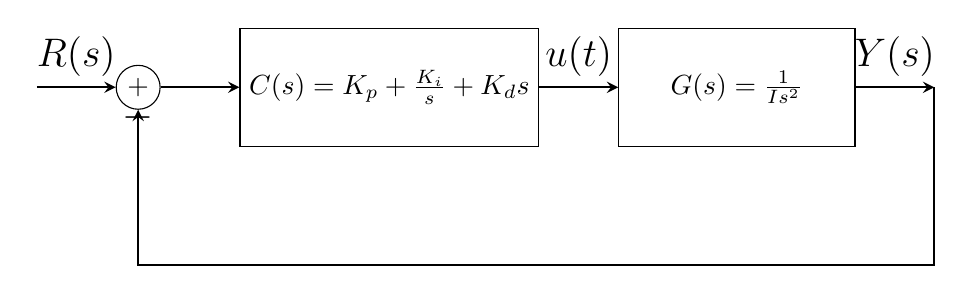
\begin{tikzpicture}[auto, node distance=1cm]

    % Nodes
    \node [sum] (sum) {$+$};
   \node [block, right=of sum] (controller) {$C(s) = K_p + \frac{K_i}{s} + K_d s$};
    \node [block, right=of controller] (quad) {$G(s) = \frac{1}{I s^2}$};
    \node [coordinate, right=of quad] (output) {};
    \node [coordinate, below=1.5cm of quad] (feedback) {};
    \node [coordinate, left=of sum] (input) {};

    % Arrows
    \draw [arrow] (input) -- node{\Large$R(s)$} (sum);
    \draw [arrow] (sum) -- (controller);
    \draw [arrow] (controller) -- node{\Large$u(t)$} (quad);
    \draw [arrow] (quad) -- node{\Large$Y(s)$} (output);
    \draw [arrow] (output) |- (feedback) -| node[pos=0.9, above]{\Large$-$} (sum);

\end{tikzpicture}
\end{center}
    \caption{Malha de controle fechada quadrotor}
    \fonte{Elaborado pelo autor.}
    \label{fig:malha_fechada_drone}
\end{figure}
Onde $G(s)$ representa a função transferência de malha aberta que modela a dinâmica do drone com 4 rotores, sendo $I$  momento de inércia sob os respectivos eixos. $R(s)$ indica a entrada de referência, ou seja, os ângulos roll,pitch e yaw desejados. $Y(s)$ representa a saída obtida a partir dos sensores IMU do drone, que são retroalimentados para computação do erro, ajustando a entrada do controlador.

%\noindent\textbf{Sugestão de Ilustração:} Diagrama em blocos de um sistema de controle de voo de UAV usando PID, mostrando comandos de entrada, loops de feedback e resposta dos atuadores.

\section{Enxame de VANTs}
\subsection{Definição }
Um \textbf{enxame de VANTs (Veículos Aéreos Não Tripulados)} refere-se a um grupo coordenado de drones autônomos ou semiautônomos que colaboram de forma distribuída para atingir um objetivo comum. Esses sistemas inspiram-se frequentemente em comportamentos coletivos observados na natureza, como colônias de insetos sociais, e destacam-se por sua capacidade de operar de maneira cooperativa, robusta e eficiente \cite{brambilla2013swarm, chung2018survey}.

Entre as propriedades fundamentais que caracterizam um enxame de VANTs, destacam-se:
\begin{itemize}
    \item \textbf{Arquitetura}: Esta propriedade define o local no qual as decisões do exame são processadas. As principais arquiteturas são: centralizada, descentralizada e híbrida \cite{bayndir2016review}.
    \item \textbf{Escalabilidade}: Diz respeito à capacidade do sistema de manter sua eficiência à medida que o número de agentes no enxame aumenta. Um sistema escalável é capaz de coordenar ações com dezenas ou centenas de UAVs sem comprometer o desempenho geral  \cite{chung2018survey}.
    \item \textbf{Adaptabilidade}: Representa a habilidade do enxame de reagir a mudanças no ambiente, como a presença de obstáculos, a movimentação de alvos ou a introdução de novas missões. Essa propriedade é essencial para operações em ambientes dinâmicos e não estruturados \cite{ollero2021past}.
    \item \textbf{Redundância}: Refere-se à tolerância a falhas, possibilitada pela distribuição de funções entre múltiplos agentes. Caso um ou mais drones falhem, os demais são capazes de compensar a perda e manter a continuidade da missão.
\end{itemize}

\subsection{Arquiteturas de Enxames}

As arquiteturas de controle de enxames de VANTs podem ser classificadas em três categorias principais: centralizada, descentralizada e híbrida.

Na \textbf{arquitetura centralizada}, ilustrado na figura \ref{fig:arquitetura_central}, um nó controlador central — comumente denominado estação solo — gerencia todos os VANTs, sendo responsável por enviar comandos e receber as informações coletadas pelos drones. Essa abordagem apresenta vantagens como a coordenação simplificada e a possibilidade de otimizações globais. No entanto, sofre com limitações importantes, como a existência de um ponto único de falha e baixa escalabilidade, tornando-se menos adequada para operações em larga escala ou em ambientes com conectividade instável.

A \textbf{arquitetura descentralizada}, ilustrado na figura \ref{fig:arquitetura_desc}, por sua vez, distribui a responsabilidade de tomada de decisão entre os próprios drones, que atuam com base em suas observações locais e comunicação entre pares. Para isso, cada drone deve possuir certo grau de autonomia, seja por meio de rotinas pré-programadas ou de sistemas inteligentes baseados em inteligência artificial. Essa abordagem é naturalmente mais robusta a falhas e altamente escalável. Em contrapartida, exige maior capacidade computacional embarcada nos drones e apresenta desafios adicionais de coordenação, o que pode levar a políticas subótimas em comparação com soluções centralizadas.

Por fim, a \textbf{arquitetura híbrida}, ilustrado pela figura \ref{fig:arquitetura_hibrida}, busca combinar o melhor dos dois mundos. Nela, um servidor central realiza o planejamento de alto nível, como a atribuição de tarefas, enquanto os drones executam essas tarefas de forma descentralizada, negociando trajetórias localmente e tomando decisões com base em suas próprias observações. Esse modelo permite maior flexibilidade e resiliência, ao mesmo tempo em que mantém um certo grau de controle global sobre o comportamento do enxame.

\begin{figure}[h]
    \centering
    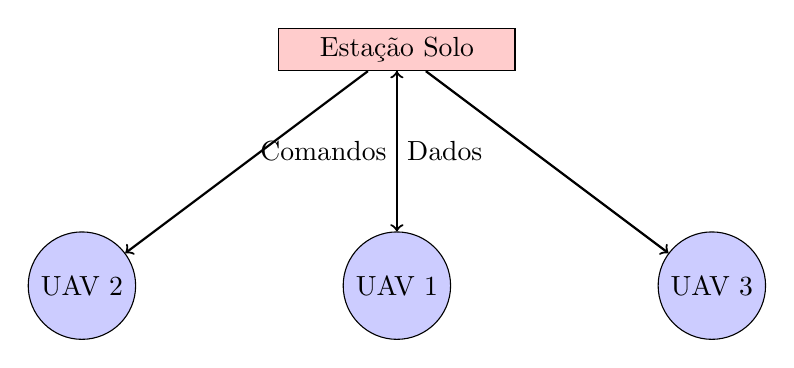
\begin{tikzpicture}[node distance=2cm]
    % Controlador Central
    \node[draw, rectangle, fill=red!20, minimum width=3cm] (central) {Estação Solo};
    % UAVs
    \node[draw, circle, fill=blue!20, below of=central, yshift=-1cm] (uav1) {UAV 1};  
    \node[draw, circle, fill=blue!20, left of=uav1, xshift=-2cm] (uav2) {UAV 2};  
    \node[draw, circle, fill=blue!20, right of=uav1, xshift=2cm] (uav3) {UAV 3};  
    % Conexões
    \draw[->, thick] (central) -- (uav1) node[midway, left] {Comandos};  
    \draw[->, thick] (central) -- (uav2);  
    \draw[->, thick] (central) -- (uav3);  
    \draw[->, thick, dashed] (uav1) -- (central) node[midway, right] {Dados};  
\end{tikzpicture}
    \caption{Arquitetura Centralizada.}
    \fonte{Elaborado pelo autor.}
    \label{fig:arquitetura_central}
\end{figure}

\begin{figure}[h]
    \centering
    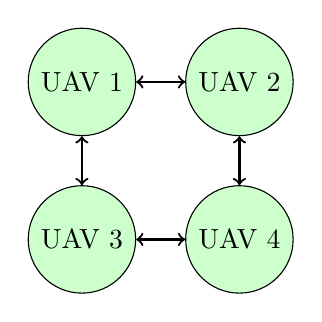
\begin{tikzpicture}[node distance=2cm]
    % UAVs
    \node[draw, circle, fill=green!20] (uav1) {UAV 1};  
    \node[draw, circle, fill=green!20, right of=uav1] (uav2) {UAV 2};  
    \node[draw, circle, fill=green!20, below of=uav1] (uav3) {UAV 3};  
    \node[draw, circle, fill=green!20, below of=uav2] (uav4) {UAV 4};  
    
    % Conexões peer-to-peer
    \draw[<->, thick] (uav1) -- (uav2);  
    \draw[<->, thick] (uav1) -- (uav3);  
    \draw[<->, thick] (uav2) -- (uav4);  
    \draw[<->, thick] (uav3) -- (uav4);  
\end{tikzpicture}
    \caption{Arquitetura Descentralizada.}
    \label{fig:arquitetura_desc}
\end{figure}


\begin{figure}[h]
    \centering
    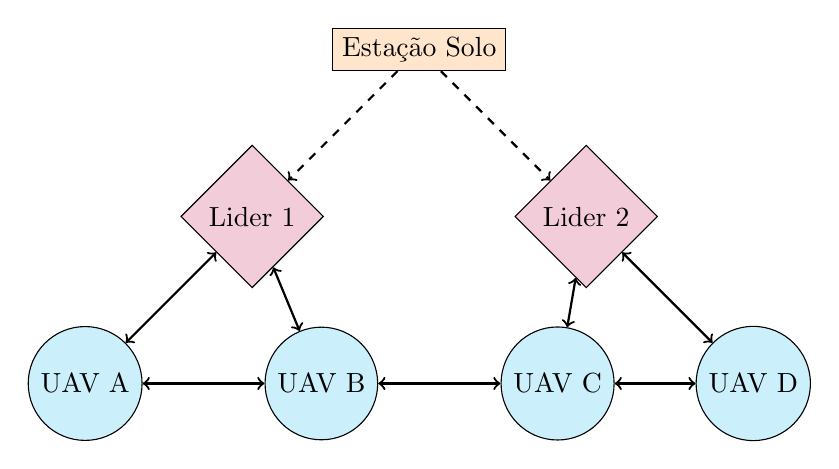
\begin{tikzpicture}[node distance=3cm]
    % Central Planner
    \node[draw, rectangle, fill=orange!20] (central) {Estação Solo};
    % Subgroup Leaders
    \node[draw, diamond, fill=purple!20, below left of=central] (lider1) {Lider 1};  
    \node[draw, diamond, fill=purple!20, below right of=central] (lider2) {Lider 2};  
    % Planner connections
    \draw[->, dashed, thick] (central) -- (lider1);  
    \draw[->, dashed, thick] (central) -- (lider2);  
    % Subgroups
    \node[draw, circle, fill=cyan!20, below left of=lider1] (uav1) {UAV A};  
    \node[draw, circle, fill=cyan!20, right of=uav1] (uav2) {UAV B};
    \node[draw, circle, fill=cyan!20, right of=uav2] (uav3) {UAV C};  
    \node[draw, circle, fill=cyan!20, below right of=lider2] (uav4) {UAV D};  
    %\node[draw, circle, fill=cyan!20, left of=uav4] (uav5) {UAV E};  
    % Peer-to-peer connections
    \draw[<->, thick] (lider1) -- (uav1); 
    \draw[<->, thick] (lider1) -- (uav2);  
    \draw[<->, thick] (uav1) -- (uav2);  
    \draw[<->, thick] (lider2) -- (uav3);  
    \draw[<->, thick] (lider2) -- (uav4);
    \draw[<->, thick] (uav3) -- (uav4);
    \draw[<->, thick] (uav2) -- (uav3);  
\end{tikzpicture}
    \caption{Arquitetura Híbrida.}
    \fonte{Elaborado pelo autor.}
    \label{fig:arquitetura_hibrida}
\end{figure}


\subsection{Aplicações e Comportamentos de Enxames de UAVs}

Os enxames de UAVs têm ganhado destaque em diversas áreas devido à sua capacidade de realizar missões cooperativas de forma eficiente, robusta e escalável. Entre as principais aplicações, destacam-se as missões de vigilância e reconhecimento, como o rastreamento de alvos e patrulhamento de fronteiras, onde múltiplos drones podem cobrir grandes áreas simultaneamente, aumentando a efetividade da missão. Em situações de resposta a desastres, os enxames são empregados em tarefas de busca e resgate e avaliação de danos, oferecendo uma solução ágil e segura para operar em ambientes perigosos ou de difícil acesso.

Na agricultura de precisão, esses sistemas são utilizados para o monitoramento em larga escala de plantações, identificação de áreas afetadas por pragas ou falta de irrigação, bem como pulverização seletiva de pesticidas. Enxames também podem ser empregados como redes de comunicação móveis, oferecendo cobertura temporária de redes 5G ou 6G em áreas remotas ou durante eventos de emergência. Em operações militares, os UAVs em enxame são aplicados em ações coordenadas, como ataques simultâneos, guerra eletrônica, reconhecimento e bloqueio de sinais, com alto grau de adaptabilidade e redundância frente a ameaças.

A execução eficiente dessas aplicações depende de comportamentos cooperativos e distribuídos, que caracterizam os sistemas de enxame. Um dos comportamentos fundamentais é a formação de voo, onde os UAVs mantêm padrões geométricos estáveis — como formações em “V” ou em grade — permitindo maior organização e controle da missão. Outro comportamento essencial é a alocação de tarefas, que envolve a distribuição dinâmica de subtarefas entre os membros do enxame, frequentemente baseada em mecanismos de leilão, heurísticas distribuídas ou aprendizado por reforço.

O planejamento colaborativo de trajetórias e desvio de obstáculos garante que os UAVs naveguem de forma eficiente, evitando colisões e otimizando rotas em ambientes dinâmicos. A tomada de decisão coletiva é outro elemento-chave, permitindo que os drones cheguem a consensos em tempo real sobre alvos prioritários ou mudanças estratégicas na missão. Por fim, a autorreconfiguração é uma capacidade crítica de resiliência, na qual o enxame reorganiza sua estrutura e ajusta seu comportamento automaticamente em resposta à falha ou perda de um ou mais UAVs, assegurando a continuidade da operação.

Dessa forma, os enxames de UAVs oferecem um paradigma promissor para a automação de missões complexas, combinando aplicações práticas variadas com uma base de comportamentos coletivos sofisticados.

\subsection{Principais Desafios no Controle de Enxames VANTs}

O controle de enxames de UAVs envolve uma série de desafios técnicos e operacionais que precisam ser superados para garantir missões bem-sucedidas, especialmente em ambientes reais e dinâmicos. Um dos principais obstáculos está na complexidade da coordenação entre múltiplos agentes. Devido à observabilidade parcial, cada UAV frequentemente só tem acesso a informações limitadas sobre o ambiente e sobre os demais membros do enxame, o que restringe sua consciência situacional e dificulta a tomada de decisões cooperativas eficazes. Essa limitação é agravada pela não estacionariedade do ambiente, típica de cenários em que múltiplos agentes aprendem ou tomam decisões simultaneamente, interferindo uns nos outros.

Outro desafio crítico está relacionado à escalabilidade do sistema. À medida que o número de drones no enxame cresce, a comunicação entre os agentes tende a gerar uma sobrecarga significativa, cujo custo computacional e de largura de banda cresce quadraticamente com o tamanho do grupo. Além disso, a coordenação em espaços de ação conjuntos de alta dimensionalidade leva à chamada maldição da dimensionalidade, dificultando o planejamento e o aprendizado de políticas eficazes.

A atuação em ambientes dinâmicos e incertos impõe a necessidade de replanejamento constante. Obstáculos móveis, alterações nas condições ambientais e movimentação de alvos exigem que os UAVs adaptem suas trajetórias e estratégias de forma reativa e em tempo real. Nessas situações, incertezas associadas a medições de sensores ou limitações na precisão dos atuadores podem comprometer a segurança e a eficácia da missão.

As restrições físicas dos drones também impõem limitações operacionais significativas. A autonomia de voo é geralmente limitada pela capacidade das baterias, o que restringe o tempo de operação contínua. Além disso, o poder computacional embarcado costuma ser reduzido, exigindo algoritmos eficientes e leves para processamento local. Isso gera um constante trade-off entre exploração (busca por novas informações) e exploração (execução de ações já conhecidas como eficazes).

Por fim, aspectos relacionados à segurança e resiliência não podem ser negligenciados. UAVs estão sujeitos a vulnerabilidades como interferência eletromagnética, ataques de spoofing e ciberataques que podem comprometer o controle, a navegação ou a integridade dos dados. Em ambientes operacionais compartilhados, a presença de agentes adversários ou aeronaves desconhecidas representa uma ameaça adicional que deve ser considerada nos mecanismos de controle e decisão coletiva.

Esses desafios exigem abordagens inovadoras em áreas como aprendizado por reforço multiagente, controle distribuído, comunicações seguras e design de arquiteturas robustas para garantir que os enxames de UAVs possam operar de forma autônoma, eficiente e segura em cenários cada vez mais complexos.



\section{Fundamentos do Aprendizado por Reforço}

O Aprendizado por Reforço (Reinforcement Learning - RL) é um paradigma de aprendizado de máquina inspirado pela psicologia comportamental, onde um agente aprende a tomar decisões interagindo com um ambiente para maximizar recompensas cumulativas. Diferentemente do aprendizado supervisionado, no qual os modelos aprendem com dados rotulados, o RL depende de interações por tentativa e erro para descobrir estratégias ótimas. Segundo \cite{sutton2018reinforcement}, os conceitos fundamentais no RL são descritos como segue.
\begin{figure}[!h]
	\centering
	\includegraphics[scale=0.6]{fig/rl_loop_uav.png}
	\caption{Exemplo de diagrama esquemático sistema RL com agente VANT}
	\fonte{Autor.}
    \label{fig:rl_diagram}
\end{figure}

\subsection{Agente}
O agente é o tomador de decisões dentro do framework de RL. Ele interage com o ambiente executando ações e aprende uma política (\textit{policy})—um mapeamento entre estados e ações que determina a tomada de decisões do agente. A política é o núcleo central do agente, de modo esta determina o comportamento do agente. Portanto a fase de treinamento do agente, consiste em encontrar uma política que maximize a recompensa acumulada (retorno) esperada ao longo do período de atuação do agente.
A figura \ref{fig:rl_diagram} ilustra o fluxo de interação entre o agente e o ambiente. 
\subsection{Ambiente}
O ambiente representa tudo fora do agente com o qual ele interage. Ele fornece ao agente um estado ou observação, que é uma representação da situação atual que o agente é capaz de perceber, e responde às ações do agente mudando para um novo estado e oferecendo feedback em forma de recompensa. 
\begin{definition}[Framework RL]
Formalmente, o framwork de RL é modelado como um Processo de Decisão de Markov (MDP), definido pela tupla $\langle S,A,P,R \rangle$ onde:
\begin{itemize}
    \item (\(S\)): Conjunto denominado espaço de estados. Neste trabalho o espaço de estados são o conjunto de observações que o drone obtém do ambiente. Informações como: pose do drone no espaço, pontos de nuvem das leituras do sensor LiDAR, imagens das câmeras do drone, GPS (latitude e longitude).
    \item (\(A\)): Conjunto denominado espaço de ações.
    \item \(P(s_{t+1}|s_t, a_t)\): Uma função de transição , que define a probabilidade de transição para o estado \(s_{t+1}\) ao realizar a ação \(a_t\) no estado \(s_t\).
    \item \(R(s, a)\): Função de recompensa, que atribui um valor escalar às transições.
\end{itemize}
    
\end{definition}

\subsection{Recompensa}
A recompensa é um sinal de feedback escalar que quantifica o benefício imediato de uma ação tomada pelo agente. Este é o principal sinal que orienta o processo de aprendizado do agente. O objetivo do agente é maximizar a recompensa cumulativa (retorno) recebida ao longo do tempo. Isso envolve equilibrar recompensas imediatas e ganhos potenciais de longo prazo. O tipo de retorno mais utilizado é o \textbf{retorno esperado de horizonte infinito}, limitado o fator de desconto \(\gamma \in (0,1)\), definido como:
\begin{equation}
    R(\tau) = \sum_{t=0}^{\infty} \gamma^{t}r_t  
\end{equation}
onde $R(s_t, a_t)=r_t$ e $\tau=(s_0,a_0,s_1,a_1,...)$ representa um histórico de sequência de estados e ações tomadas no ambiente.
\subsection{Política}
A política (\(\pi\)) define o comportamento do agente. É uma função ou distribuição de probabilidade que mapeia estados para ações. Políticas podem ser determinísticas (\(a_t = \pi(s_t) \)) ou estocásticas \(\pi(a_t|s_t) \in [0,1]\).

\subsection{Problema central em RL}
O objetivo principal do aprendizado por reforço, consiste então, em selecionar uma política $\pi$ que maximize a função de retorno esperada. Para definir matematicamente esse problema é preciso estabelecer o conceito de trajetória, $\tau=(s_0,a_0,s_1,a_1,...) $ que representa uma sequência de estados e ações tomadas no ambiente. Então a probabilidade de uma trajetória é definido como:
\begin{equation}
    P(\tau|\pi)=\prod_{t=0}^{T} P(s_{t+1}|s_t, a_t)\pi(a_t,s_t)
\end{equation}
O retorno esperado para uma política específica $\pi$, é denotado por $J(\pi)$ definido como:
\begin{equation}
    J(\pi)=\int_{\tau}^{} P(\tau|\pi)R(\tau) \,d\tau  
\end{equation}
O problema central de otimização no aprendizado por reforço é modelado matematicamente então como:
\begin{equation}
    \pi^*=\arg \max_\pi J(\pi)
\end{equation}

\subsection{Funções de Valor}
As funções de valor avaliam a qualidade de estados ou pares estado-ação sob uma política dada, sendo fundamentais para orientar o agente a estratégias melhores:
\begin{itemize}
    \item Função de valor de estado \(V^\pi(s)=E\): Retorno esperado ao começar no estado \(s\) e seguir a política \(\pi\).
    \item Função de valor de ação (\(Q^\pi(s, a)\)): Retorno esperado ao tomar a ação \(a\) no estado \(s\) e seguir a política \(\pi\).
\end{itemize}

\subsection{Exploração versus Aprimoramento}
Um desafio fundamental no RL é o equilíbrio entre exploração (testar novas ações para descobrir seus efeitos) e aprimoramento (Exploitation) (escolher ações já conhecidas que maximizam recompensas). Estratégias como \(\epsilon\)-gananciosa (\(\epsilon\)-greedy) e Bound de Confiança Superior (UCB, do inglês Upper Confidence Bound) tratam deste equilíbrio ao combinar a necessidade do agente de coletar informações e alcançar altas recompensas.

\subsection{Métodos de Aprendizado}

Os algoritmos de Aprendizado por Reforço (Reinforcement Learning, RL) podem ser classificados em três grandes categorias, cada uma com diferentes estratégias para lidar com a dinâmica do ambiente e o processo de tomada de decisão.

Os métodos \textbf{model-free} (sem modelo) não exigem conhecimento prévio das funções de transição e recompensa do ambiente. Em vez disso, eles aprendem diretamente a política ou a função de valor a partir das interações com o ambiente. Dentro desta categoria, destacam-se os métodos baseados em valores, como o \textit{Q-Learning}, que busca estimar a função de valor de ação \( Q(s, a) \) para selecionar ações que maximizem a recompensa acumulada. Uma extensão poderosa dessa abordagem é o uso de redes neurais profundas, resultando nos \textit{Deep Q-Networks (DQNs)}, que permitem aplicar Q-Learning em ambientes com grandes espaços de estados, como aqueles representados por imagens ou sensores de alta dimensão.

Por outro lado, os métodos \textbf{model-based} (baseados em modelo) tentam construir uma representação explícita do ambiente, aprendendo suas dinâmicas — isto é, como os estados evoluem e quais recompensas são associadas às ações. Esses métodos permitem o uso de técnicas de planejamento, como simulações internas (\textit{rollouts}), para prever consequências futuras antes de agir, o que pode acelerar o processo de aprendizado e melhorar a amostragem de dados. Contudo, são mais sensíveis a erros no modelo aprendido.

A terceira categoria compreende os \textbf{métodos de otimização de política}, que consistem em atualizar diretamente os parâmetros da política com base em gradientes estimados da função objetivo. Ao invés de depender da estimativa de funções de valor, esses métodos otimizam diretamente a probabilidade de selecionar boas ações. Entre os algoritmos mais representativos dessa abordagem estão o \textit{Proximal Policy Optimization (PPO)} e o \textit{Trust Region Policy Optimization (TRPO)}, ambos amplamente utilizados por sua estabilidade e eficácia em tarefas com múltiplas etapas e ambientes contínuos.

Em sistemas multiagente, essas categorias se mantêm, mas a complexidade aumenta devido à não estacionariedade introduzida pela presença de múltiplos agentes aprendendo simultaneamente. A escolha do método adequado, portanto, deve considerar a natureza do ambiente, a escalabilidade e os objetivos do controle distribuído no sistema de enxame.


%Conforme discutido em \cite{sutton2018reinforcement}, o Aprendizado por Reforço tem sido amplamente aplicado em áreas como robótica, jogos e sistemas autônomos, destacando-se como uma abordagem poderosa, porém desafiadora, devido a problemas como recompensas esparsas e alta dimensionalidade de espaços de estado.

\section{Aprendizado por Reforço Multiagente (MARL)}
O Aprendizado por Reforço Multiagente (MARL) estende o aprendizado por reforço de agente único para ambientes onde múltiplos agentes aprendem a interagir e colaborar. 

\begin{definition}[Framework MARL]
Formalmente, o MARL é modelado como um \textbf{Jogo de Markov} \cite{LITTMAN}, definido pela tupla \(\langle \mathcal{N}, \mathcal{S}, \{\mathcal{A}^i\}, \mathcal{P}, \{\mathcal{R}^i\}, \gamma \rangle\), onde:
\begin{itemize}
    \item \(\mathcal{N}\): Conjunto de \(n\) agentes.
    \item \(\mathcal{S}\): Espaço de estados compartilhado.
    \item \(\mathcal{A}^i\): Espaço de ações do agente \(i\).
    \item \(\mathcal{P}(s' | s, \mathbf{a})\): Probabilidade de transição para o estado \(s'\) dada a ação conjunta \(\mathbf{a} = (a^1, \dots, a^n)\).
    \item \(\mathcal{R}^i(s, \mathbf{a})\): Função de recompensa do agente \(i\).
    \item \(\gamma\): Fator de desconto.
\end{itemize}
    
\end{definition}

Diferentemente do RL de agente único, no MARL os agentes devem equilibrar recompensas individuais com objetivos coletivos, gerando desafios únicos:
\begin{itemize}
    \item \textbf{Não Estacionariedade}: Políticas dos agentes mudam concorrentemente, violando a suposição de Markov.%\cite{foerster2017stabilising}.
    \item \textbf{Atribuição de Crédito}: Dificuldade em associar sucessos/falhas globais a ações individuais.% \cite{wei2021credit}.
    \item \textbf{Observabilidade Parcial}: Agentes observam apenas estados locais \(o^i \subset \mathcal{S}\).% \cite{oliehoek2016concise}.
\end{itemize}

\subsection{Abordagens Algorítmicas em MARL}  
Os desafios de coordenação em enxames de UAVs exigem estratégias de \textit{Multi-Agent Reinforcement Learning} (MARL) que equilibrem escalabilidade, eficiência e adaptabilidade. A literatura especializada propõe três paradigmas principais para lidar com essas demandas:  
\begin{enumerate}
    \item \textbf{Aprendizado Independente (IQL - Independent Q-Learning)} \cite{tan1993multi}:  
    Nesta abordagem, cada agente aprende uma função de valor \(Q^i(o^i, a^i)\) de forma totalmente descentralizada, ignorando as ações e observações dos demais. A simplicidade computacional do IQL o torna escalável para grandes enxames, mas a falta de modelagem explícita das interdependências entre agentes frequentemente resulta em coordenação subótima, especialmente em tarefas que exigem sincronização ou divisão de recursos \cite{tan1993multi}.  
    
    \item \textbf{Treinamento Centralizado com Execução Descentralizada (CTDE)} \cite{kraemer2016multi}:  
    Para superar as limitações do IQL, métodos como o QMIX 
    utilizam informações globais durante o treinamento (e.g., estados agregados do enxame) enquanto mantêm políticas de execução baseadas em observações locais. O QMIX, por exemplo, impõe uma fatorização monotônica das funções-Q individuais (\( \partial Q_{\text{total}} / \partial Q^i \geq 0 \)), garantindo que a maximização dos Q-valores locais corresponda à otimização do valor global do enxame. Essa estratégia é particularmente eficaz em missões de vigilância cooperativa, onde a coordenação tácita é crítica \cite{rashid2018qmix}.  

    \item \textbf{Treinamento e Execução Totalmente Descentralizados (DTDE)} \cite{schulman2017}:  
    Algoritmos como o IPPO (\textit{Independent Proximal Policy Optimization}) priorizam a escalabilidade extrema, permitindo que cada agente treine e execute políticas baseadas apenas em observações locais. Embora adequado para enxames massivos em ambientes com restrições de comunicação, o DTDE enfrenta dificuldades em cenários que exigem sincronização fina entre agentes, como formação dinâmica em espaços congestionados \cite{schulman2017}.  

\end{enumerate}

Dentre os algoritmos de Aprendizado por Reforço Multiagente (MARL) mais consolidados para controle de enxames, destacam-se:

\begin{itemize}
    \item \textbf{MAPPO} \cite{yu2021mappo}: Baseado no paradigma CTDE (Centralized Training with Decentralized Execution), combina redes \textit{actor-critic} com críticos centralizados, sendo especialmente eficaz em espaços de ação contínuos — ideal para ajustes precisos de trajetória em UAVs.
    
    \item \textbf{VDN} \cite{sunehag2017value}: Decompõe o valor global do enxame em uma soma de Q-valores individuais, o que facilita a otimização distribuída em tarefas como a cobertura eficiente de áreas.
    
    \item \textbf{Mean-Field MARL} \cite{yang2018mean}: Modela as interações entre agentes como a média do comportamento coletivo, reduzindo significativamente a complexidade computacional — uma abordagem eficaz em cenários envolvendo centenas de UAVs.
\end{itemize}

Apesar dos avanços recentes, diversos desafios práticos ainda persistem. Algoritmos CTDE, como o QMIX, demandam comunicação de alta frequência durante o treinamento, o que limita sua aplicabilidade em sistemas com restrições energéticas \cite{rashid2018qmix}. Por outro lado, abordagens totalmente descentralizadas (DTDE) enfrentam a ``maldição da dimensionalidade'', especialmente em ambientes parcialmente observáveis \cite{schulman2017}. Além disso, a maioria das validações ocorre em simulações homogêneas, enquanto aplicações reais introduzem variabilidades como heterogeneidade de sensores, atrasos de comunicação e falhas de hardware não modeladas \cite{yang2018mean}.

Nesse contexto, a integração de MARL com técnicas de \textit{transfer learning} e arquiteturas neuro-simbólicas desponta como uma estratégia promissora para superar essas limitações e aproximar a pesquisa do uso prático em campo.


\subsection{Multi-Agent Proximal Policy Optimization (MAPPO)}
\label{subsec:mappo}

O \textit{Multi-Agent Proximal Policy Optimization} (MAPPO) é um algoritmo de aprendizado por reforço multiagente que estende o método \textit{Proximal Policy Optimization} (PPO), proposto originalmente por Schulman et al.~\cite{schulman2017ppo}, para cenários cooperativos com múltiplos agentes. O MAPPO foi formalizado por Yu et al.~\cite{yu2021mappo} como uma alternativa estável e escalável para problemas caracterizados por observabilidade parcial e necessidade de coordenação, como aqueles encontrados em sistemas de enxames de veículos aéreos não tripulados.

O MAPPO adota o paradigma de \textit{Centralized Training with Decentralized Execution} (CTDE), no qual o treinamento das políticas é realizado de forma centralizada, enquanto a execução ocorre de maneira descentralizada. Nesse contexto, cada agente executa uma política local baseada apenas em suas observações individuais, ao passo que, durante o treinamento, um crítico centralizado pode explorar informações globais do sistema para estimar funções de valor mais informativas, reduzindo a variância das atualizações de política.

Considere um sistema composto por $N$ agentes. Cada agente $i$ observa, no instante $t$, uma observação local $\mathbf{o}_i(t)$ e executa uma ação $\mathbf{a}_i(t)$ de acordo com uma política estocástica parametrizada $\pi_\theta$, compartilhada entre todos os agentes:
\[
\mathbf{a}_i(t) \sim \pi_\theta(\mathbf{a}_i \mid \mathbf{o}_i).
\]
O compartilhamento de parâmetros entre agentes, prática adotada no MAPPO, contribui para a escalabilidade do algoritmo e para a emergência de comportamentos cooperativos simétricos~\cite{yu2021mappo}.

Durante o treinamento, o MAPPO emprega um crítico centralizado $V_\phi$, que estima o valor esperado do retorno a partir de um estado global ou de uma concatenação das observações dos agentes:
\[
V_\phi(\mathbf{s}(t)) \approx \mathbb{E}\!\left[ \sum_{k=0}^{\infty} \gamma^k r(t+k) \,\middle|\, \mathbf{s}(t) \right],
\]
onde $\mathbf{s}(t)$ representa o estado global disponível apenas durante o treinamento, $r(t)$ é a recompensa compartilhada e $\gamma \in (0,1)$ é o fator de desconto.

O MAPPO herda do PPO a função objetivo baseada em \textit{clipping}, projetada para limitar variações excessivas na política durante as atualizações e garantir estabilidade no processo de aprendizado~\cite{schulman2017ppo}. A função objetivo otimizada pelo ator é dada por:
\[
\mathcal{L}^{\text{CLIP}}(\theta) =
\mathbb{E}_t \left[
\min \left(
\rho_t(\theta) \hat{A}_t,\;
\mathrm{clip}\big(\rho_t(\theta), 1-\epsilon, 1+\epsilon\big)\hat{A}_t
\right)
\right],
\]
em que $\rho_t(\theta) = \frac{\pi_\theta(\mathbf{a}_i(t)\mid \mathbf{o}_i(t))}{\pi_{\theta_{\text{old}}}(\mathbf{a}_i(t)\mid \mathbf{o}_i(t))}$ é a razão de probabilidade entre a política atual e a anterior, $\epsilon$ é o parâmetro de \textit{clipping} e $\hat{A}_t$ representa a estimativa da vantagem.

A estimativa da vantagem é tipicamente calculada por meio do método de \textit{Generalized Advantage Estimation} (GAE), introduzido por Schulman et al.~\cite{schulman2016gae}, que combina viés e variância de forma controlada:
\[
\hat{A}_t = \sum_{l=0}^{\infty} (\gamma \lambda)^l \delta_{t+l},
\quad
\delta_t = r(t) + \gamma V_\phi(\mathbf{s}(t+1)) - V_\phi(\mathbf{s}(t)),
\]
onde $\lambda \in (0,1)$ é o parâmetro de suavização temporal.

Ao combinar a estabilidade do PPO com o formalismo CTDE, o MAPPO fornece uma abordagem robusta para aprendizado por reforço multiagente em ambientes contínuos e parcialmente observáveis, sendo amplamente adotado em tarefas cooperativas complexas, incluindo controle de formações e coordenação de enxames robóticos~\cite{yu2021mappo}.

\begin{figure}[H]
\centering
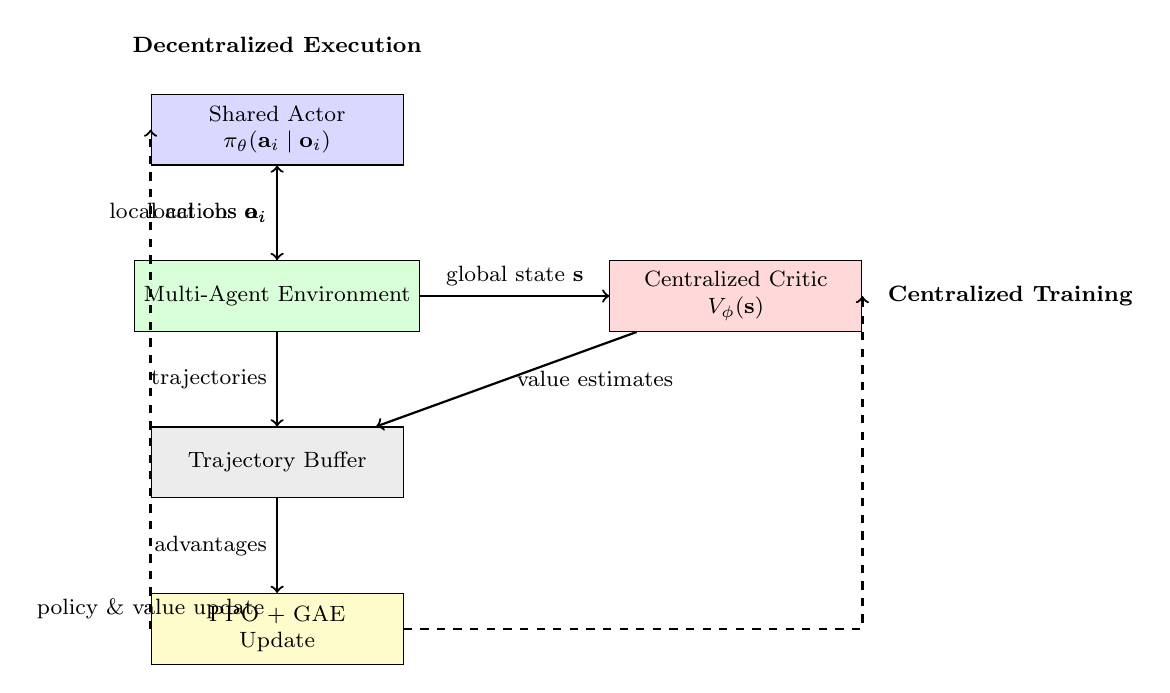
\begin{tikzpicture}[
    node distance=1.2cm and 2.4cm,
    actor/.style={rectangle, draw, fill=blue!15, minimum width=3.2cm, minimum height=0.9cm, align=center},
    critic/.style={rectangle, draw, fill=red!15, minimum width=3.2cm, minimum height=0.9cm, align=center},
    env/.style={rectangle, draw, fill=green!15, minimum width=3.2cm, minimum height=0.9cm, align=center},
    buffer/.style={rectangle, draw, fill=gray!15, minimum width=3.2cm, minimum height=0.9cm, align=center},
    update/.style={rectangle, draw, fill=yellow!20, minimum width=3.2cm, minimum height=0.9cm, align=center},
    arrow/.style={->, thick},
    dashedarrow/.style={->, thick, dashed},
    every node/.style={font=\footnotesize}
]

% Nodes
\node[actor] (actor) {Shared Actor\\$\pi_\theta(\mathbf{a}_i \mid \mathbf{o}_i)$};

\node[env, below=of actor] (env) {Multi-Agent Environment};

\node[critic, right=of env] (critic) {Centralized Critic\\$V_\phi(\mathbf{s})$};

\node[buffer, below=of env] (buffer) {Trajectory Buffer};

\node[update, below=of buffer] (update) {PPO + GAE\\Update};

% Execution flow
\draw[arrow] (actor) -- node[left] {local actions $\mathbf{a}_i$} (env);
\draw[arrow] (env) -- node[left] {local obs $\mathbf{o}_i$} (actor);

% Centralized training flow
\draw[arrow] (env) -- node[above] {global state $\mathbf{s}$} (critic);
\draw[arrow] (critic) -- node[right] {value estimates} (buffer);

\draw[arrow] (env) -- node[left] {trajectories} (buffer);

\draw[arrow] (buffer) -- node[left] {advantages} (update);

\draw[dashedarrow] (update.west) -| node[above] {policy \& value update} (actor.west);
\draw[dashedarrow] (update.east) -| (critic.east);

% Labels
\node[above=0.4cm of actor] {\textbf{Decentralized Execution}};
\node[right=0.2cm of critic] {\textbf{Centralized Training}};

\end{tikzpicture}
\caption{Fluxograma do treinamento MAPPO no paradigma de Treinamento Centralizado com Execução Descentralizada (CTDE). Durante a execução, cada agente utiliza apenas observações locais por meio de uma política compartilhada. Durante o treinamento, um crítico centralizado explora o estado global para atualizar os parâmetros da política e da função de valor.}
\label{fig:ctde_flow}
\end{figure}

\subsection{Descrição Algorítmica do MAPPO}

O Algoritmo~\ref{algo:mappo} apresenta o fluxo geral de treinamento do MAPPO no paradigma de \textit{Centralized Training with Decentralized Execution} (CTDE). Durante a coleta de experiências, cada agente executa ações de forma descentralizada a partir de observações locais, utilizando uma política compartilhada entre todos os agentes. Em contrapartida, a atualização dos parâmetros é realizada de forma centralizada, explorando um crítico global que tem acesso ao estado conjunto do sistema.

A interação com o ambiente gera trajetórias multiagentes compostas por observações locais, ações e recompensas compartilhadas, que são armazenadas em um buffer de experiências. A partir dessas trajetórias, são estimadas as vantagens utilizando o método de \textit{Generalized Advantage Estimation} (GAE). O ator é então atualizado por meio da função objetivo com \textit{clipping} do PPO, enquanto o crítico é otimizado por regressão sobre o retorno esperado.

Esse procedimento permite reduzir a variância das atualizações de política, ao mesmo tempo em que preserva a execução descentralizada, característica fundamental para aplicações em sistemas distribuídos, como enxames de VANTs.

\begin{algorithm}[H]
\caption{Multi-Agent Proximal Policy Optimization (MAPPO)}
\label{algo:mappo}
\begin{algorithmic}[1]
\STATE Inicializar política compartilhada $\pi_\theta$ e crítico centralizado $V_\phi$
\FOR{episódio = $1$ até $N_{\text{episódios}}$}
    \STATE Inicializar ambiente multiagente
    \STATE Inicializar buffer de trajetórias $\mathcal{B} \leftarrow \emptyset$
    \FOR{passo = $1$ até $T$}
        \FOR{cada agente $i = 1,\dots,N$}
            \STATE Observar estado local $\mathbf{o}_i(t)$
            \STATE Amostrar ação $\mathbf{a}_i(t) \sim \pi_\theta(\cdot \mid \mathbf{o}_i(t))$
        \ENDFOR
        \STATE Executar ação conjunta $\mathbf{a}(t)$ no ambiente
        \STATE Obter recompensa compartilhada $r(t)$ e novas observações
        \STATE Armazenar $(\mathbf{o}(t), \mathbf{a}(t), r(t), \mathbf{o}(t+1))$ em $\mathcal{B}$
    \ENDFOR
    \STATE Estimar vantagens $\hat{A}_t$ usando GAE
    \FOR{época de atualização = $1$ até $K$}
        \STATE Atualizar crítico: $\phi \leftarrow \phi - \alpha_V \nabla_\phi \mathcal{L}_V$
        \STATE Atualizar ator via PPO:
        \[
        \theta \leftarrow \theta - \alpha_\pi \nabla_\theta 
        \mathbb{E}\big[\min(\rho_t \hat{A}_t,
        \mathrm{clip}(\rho_t,1-\epsilon,1+\epsilon)\hat{A}_t)\big]
        \]
    \ENDFOR
\ENDFOR
\end{algorithmic}
\end{algorithm}




%\subsection{MARL para Enxames de VANTs}
%O MARL é particularmente adequado para controle de enxames de UAVs devido à sua capacidade de:
%\begin{itemize}
%    \item Escalar para grandes populações de agentes via treinamento e execução descentralizada (\textit{Decentralized Training and Decentralized Execution} - DTDE).
%    \item Otimizar objetivos globais (ex: rastreamento de alvos) através de coordenação emergente.
%    \item Adaptar-se a ambientes dinâmicos via aprendizado online.
%\end{itemize}


\section{Máquinas de Recompensa}

\subsection{Conceitos sobre RMs}

As \textit{Reward Machines} (RMs) consistem em um formalismo baseado em autômatos finitos que visa estruturar e modularizar funções de recompensa em problemas de aprendizado por reforço (RL). Tradicionalmente, as funções de recompensa são tratadas como "caixas-pretas", sendo acessadas pelo agente apenas para consulta pontual de valores. As RMs propõem uma abordagem diferente, em que a estrutura interna da função de recompensa é explicitada ao agente, permitindo que ele utilize tal conhecimento para acelerar e modular o processo de aprendizado \cite{rm_marl}.

\begin{definition}[Máquina de Recompensas]
Uma \textbf{Reward Machine} (RM) é uma tupla $M = \langle U, u_0, F, \delta_u, \delta_r, P \rangle$, onde:
\begin{itemize}
    \item $U$ é um conjunto finito de estados da máquina de recompensa;
    \item $u_0 \in U$ é o estado inicial da RM;
    \item $F \subseteq U$ é o conjunto de estados terminais;
    \item $P$ é um conjunto de proposições que descrevem eventos observáveis no ambiente;
    \item $\delta_u : U \times 2^{P} \rightarrow U \cup F$ é a função de transição da RM, que define a mudança de estados da RM com base nos eventos observados;
    \item $\delta_r : U \times 2^{P} \rightarrow \mathbb{R}$ é a função de recompensa que associa uma recompensa real a cada transição da RM.
\end{itemize}
\end{definition}


Formalmente, uma RM é composta por um conjunto de estados $U$, uma função de transição $\delta_u$, e uma função de recompensa $\delta_r$. O agente, ao interagir com o ambiente, transita não apenas pelos estados do ambiente, mas também pelos estados da RM, de acordo com eventos de alto nível observados no ambiente e definidos via uma função de rotulagem $L$. Cada transição na RM pode especificar uma recompensa distinta, tornando possível descrever recompensas não-Markovianas ou recompensas que dependem de propriedades temporais do histórico do agente.




A principal vantagem das RMs está na capacidade de decompor missões complexas em \textit{subtarefas} modulares, facilitando a especificação de propriedades temporais como sequências de eventos, loops e condicionais. Por exemplo, em um cenário de entrega de pacotes com UAVs, uma RM pode especificar que primeiro o agente deve "localizar o alvo" e, em seguida, "entregar o pacote" em outra localização, premiando adequadamente cada etapa.

%Além de aumentar a expressividade da função de recompensa, as RMs possibilitam a aplicação de técnicas de \textit{shaping} de recompensas e decomposição hierárquica de políticas. Técnicas como Q-learning para RMs (QRM) ou abordagens de \textit{counterfactual reasoning} (CRM) se beneficiam diretamente da estrutura exposta pelas RMs, resultando em melhor eficiência amostral e políticas mais robustas em ambientes parcialmente observáveis ou com recompensas esparsas.

Por fim, as RMs possuem o mesmo poder expressivo de linguagens regulares, sendo capazes de capturar propriedades temporais similares às especificadas por lógicas como LTL (\textit{Linear Temporal Logic}), oferecendo uma alternativa prática e compacta para a especificação de tarefas em RL.

\begin{definition}[MDP com Reward Machine (MDPRM)]
Um \textbf{MDP com Reward Machine} é uma tupla estendida $T = \langle S, A, p, \gamma, P, L, M \rangle$, onde:
\begin{itemize}
    \item $S$ é o conjunto finito de estados do ambiente;
    \item $A$ é o conjunto finito de ações disponíveis ao agente;
    \item $p: S \times A \times S \rightarrow [0,1]$ é a função de transição estocástica do ambiente;
    \item $\gamma \in (0,1]$ é o fator de desconto;
    \item $P$ é o conjunto de proposições de eventos (compartilhado com a RM);
    \item $L : S \times A \times S \rightarrow 2^{P}$ é a função de rotulagem, que associa a cada transição no ambiente um conjunto de proposições verdadeiras;
    \item $M = \langle U, u_0, F, \delta_u, \delta_r, P \rangle$ é a \textit{Reward Machine} associada.
\end{itemize}
\end{definition}

\begin{figure}[H]
    \centering
    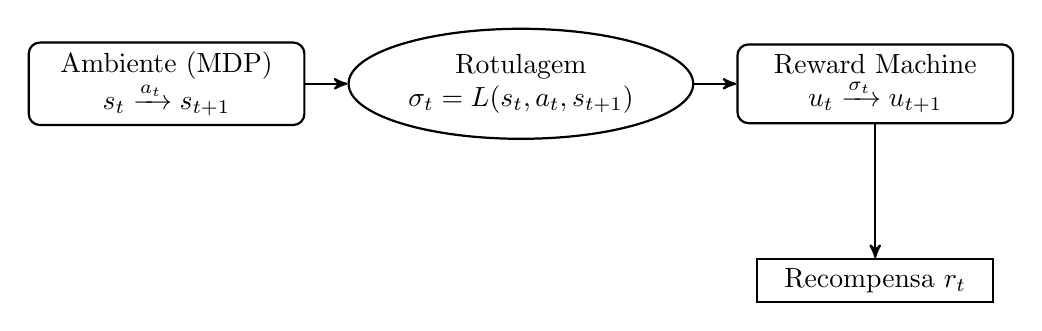
\begin{tikzpicture}[->, >=stealth', node distance=3cm, auto, thick, align=center]
        % Ambiente
        \node[draw, rectangle, rounded corners, minimum width=3.5cm, minimum height=1cm] (env) {Ambiente (MDP) \\ $s_t \xrightarrow{a_t} s_{t+1}$};

        % Label function
        \node[draw, ellipse, right of=env, node distance=4.5cm] (label) {Rotulagem \\ $\sigma_t = L(s_t, a_t, s_{t+1})$};

        % Reward Machine
        \node[draw, rectangle, rounded corners, right of=label, node distance=4.5cm, minimum width=3.5cm, minimum height=1cm] (rm) {Reward Machine \\ $u_t \xrightarrow{\sigma_t} u_{t+1}$};

        % Reward output
        \node[draw, rectangle, below of=rm, node distance=2.5cm, minimum width=3cm] (reward) {Recompensa $r_t$};

        % Arrows
        \path (env) edge node[above] {} (label);
        \path (label) edge node[above] {} (rm);
        \path (rm) edge node[right] {} (reward);

        % Feedback loop to agent (optional)
       % \draw[->, dashed] (reward.west) to[out=180,in=-90] node[left] {Reforço para o agente} ([yshift=-1cm]env.south);

    \end{tikzpicture}
    \caption{Fluxo de interação entre o ambiente, a função de rotulagem e a Reward Machine.}
    \fonte{Adapatado de \cite{rm_marl}}
    \label{fig:mdprm}
\end{figure}
A figura \ref{fig:mdprm} ilustra como a função de rotulagem $L$ realiza a interface entre a transição dos estados do ambiente com a transição de estados da máquina de recompensa. O agente ao realizar a ação $a_t$ muda o estado do ambiente de $s_t $ para $s_{t+1}$. A função rotulagem $L$ transforma a 3-tupla $(s_t,a_t,s_{t+1})$ em uma transição $\sigma_t$ da máquina de recompensa alterando seu estado de $u_t$ para $u_{t+1}$, fornecendo a recompensa $r_t$ para o agente.
\subsection{Exemplo RM: Grid World}
\begin{figure}[!h]
	\centering
	\includegraphics[scale=0.9]{fig/RM_grid_world.png}
	\caption{Exemplo de RM para o ambiente GridWorld}
	\fonte{Extraído de \cite{rm_marl}}
    \label{fig:rm_grid}
\end{figure}
A figura \ref{fig:rm_grid} mostra um exemplo de máquina de recompensas para o ambiente \textit{GridWorld}. Neste ambiente o agente consegue se movimentar nas direções cardinais, seu objetivo consiste em obter o café e o jornal acessando as posições em que os itens se encontram e entrega-las até a posição do escritório $o$. Este é um exemplo simples no qual há um requisito temporal para as sequências das atividades que o agente deve completar antes de chegar até o seu destino final. Os rótulos sobre as setas de transições da máquina de recompensa na figura a direita indicam em forma de 2-tupla respectivamente a função de rotulagem e o retorno esperado pelo agente. Por exemplo o sob o estado $u_1$ o rótulo $<\neg o \land \neg*,0>$ indica que quando o agente movimenta-se para uma posição que não é o escritório $(o)$ e também não possui um obstáculo $(*)$ ele recebe a recompensa escalar 0 e mantém a máquina de estados no estado $u_1$.
%\chapter{Trabalhos Relacionados}
Neste capítulo, são apresentados os trabalhos identificados a partir de uma revisão sistemática da literatura. É importante ressaltar que os trabalhos incluídos aqui representam apenas um extrato da literatura acadêmica, servindo como referencial para o desenvolvimento desta dissertação.
\section{Revisão Sistemática da Literatura}
Esta revisão foca especificamente em abordagens baseadas em IA, particularmente Aprendizado por Reforço (RL) e Aprendizado Profundo (DL), em vez de oferecer uma análise ampla dos métodos tradicionais. Esse foco é motivado pelo crescente consenso na literatura de que as técnicas de IA são essenciais para superar as limitações das abordagens convencionais na adaptação a ambientes complexos e dinâmicos. Os VANTs modernos agora são equipados com processadores poderosos e sensores avançados, permitindo tomada de decisão em tempo real e ajustes dinâmicos às mudanças ambientais. Os objetivos que esta revisão busca enfatizar são:  %Métodos tradicionais, como técnicas baseadas em regras ou otimização estática, frequentemente carecem da flexibilidade necessária para lidar com mudanças imprevisíveis ou condições não estruturadas.

%Avanços recentes nos algoritmos de RL e DL, aliados a melhorias significativas nas capacidades computacionais e sensoriais embarcadas em VANTs, reforçaram ainda mais o potencial transformador das abordagens baseadas em IA. Os VANTs modernos agora são equipados com processadores poderosos e sensores avançados, permitindo tomada de decisão em tempo real e ajustes dinâmicos às mudanças ambientais. Essas capacidades aprimoradas possibilitam que os métodos baseados em IA alcancem níveis superiores de adaptabilidade, escalabilidade e robustez em diversos cenários operacionais. Ao concentrar-se nessas metodologias avançadas, esta revisão busca fornecer insights práticos sobre como a IA pode aprimorar o desempenho de enxames de VANTs, tanto em ambientes reais quanto em simulações de alta fidelidade, abordando desafios que as técnicas tradicionais não conseguem superar de forma eficaz.

\begin{itemize}
    \item \textbf{Validação em Ambientes Reais e Simulações de Alta Fidelidade}: Destacando métodos testados em enxames de VANTs físicos ou simuladores 3D avançados para fornecer insights práticos sobre sua viabilidade.
    \item \textbf{Contribuições Específicas para Tarefas}: Detalhando como os métodos de RL e DL abordam tarefas essenciais do enxame, como planejamento de trajetória, prevenção de colisões e controle de formação em ambientes reais ou simulados.
    \item \textbf{Métricas de Desempenho e Trade-Offs}: Avaliando escalabilidade, eficiência energética e robustez, além de identificar compromissos e desafios na implementação de sistemas de enxame baseados em IA.
\end{itemize}
 
\section{Questões da RSL}
Os questionamentos que guiaram a RSL foram:
\begin{enumerate}
    \item \textbf{RQ1}: Como as abordagens de aprendizado por reforço (RL) e aprendizado profundo (DL) podem lidar com os desafios de escalabilidade, adaptabilidade e robustez em sistemas de enxame de VANTs?

    \item \textbf{RQ2}: Quais são os algoritmos de RL e DL mais avançados utilizados em sistemas de enxame de VANTs?

    \item \textbf{RQ3}: Quais são as contribuições específicas de RL e DL para tarefas de enxame de VANTs, como planejamento de trajetória, prevenção de obstáculos e controle de formação?

    \item \textbf{RQ4}: Quais métricas de desempenho são comumente utilizadas para avaliar sistemas de enxame de VANTs?

    \item \textbf{RQ5}: Como as abordagens de RL e DL melhoram a eficiência energética, a taxa de sucesso das missões e a adaptabilidade em sistemas de enxame de VANTs?

    \item \textbf{RQ6}: Até que ponto os métodos de RL e DL são validados em cenários reais de enxames de VANTs e quais são os desafios para reduzir a lacuna entre simulação e implementação?
\end{enumerate}
 
\section{Metodologia}
 O processo de busca para esta revisão sistemática foi orientado pelo framework PICO (População, Intervenção, Comparação, Resultado), uma metodologia amplamente estabelecida e utilizada em revisões sistemáticas para desenvolver estratégias de busca abrangentes e focadas. O framework PICO facilitou a criação de uma string de busca projetada para capturar os estudos mais relevantes na área de sistemas de enxame de VANTs baseados em IA.

 \begin{table}[ht]
\centering
\caption{Construção da string de busca utilizando o framework PICO}
\begin{tabularx}{\columnwidth}{|c|c|X|}
\hline
\textbf{Letra} & \textbf{Componente} & \textbf{Termos buscados} \\ \hline
P              & Population          & “Multi UAV”, “autonomous drones”, “UAV Swarm”, “unmanned aerial vehicle swarm”, “autonomous UAV” \\ \hline
I              & Intervention        & “multi-agent reinforcement learning”, “Deep Reinforcement Learning”, “Reinforcement learning”, “Deep Learning”, “neural networks”, “MARL”, “DRL” \\ \hline
C              & Comparison          & “exploration”, “avoidance”, “planning”, “formation”, “coordination” \\ \hline
O              & Outcome             & “performance”, “efficiency”, “adaptability”, “robustness”, “scalability” \\ \hline
\end{tabularx}
\label{tab:pico_table}
\end{table}

\subsection{Base de Dados e Resultados}
Para garantir uma coleta abrangente e focada de literatura relevante para esta revisão sistemática, foram utilizadas duas bases de dados acadêmicas renomadas, \textbf{Scopus} e \textbf{IEEE Xplore}. Essas bases foram selecionadas devido à sua ampla cobertura de publicações de alta qualidade nas áreas de robótica, inteligência artificial e sistemas de VANTs.

\subsection{Definição dos Critérios}
Para garantir a seleção dos estudos mais relevantes para as questões de pesquisa e os objetivos desta revisão, um conjunto de critérios de exclusão foi definido e aplicado sistematicamente durante o processo de triagem. Esses critérios foram elaborados para filtrar estudos que não apresentem relevância, rigor metodológico ou alinhamento com o foco principal da revisão. Abaixo estão as principais razões para cada critério:

\begin{itemize}
    \item \textbf{Exclusões Baseadas no Escopo}: Estudos que não abordam enxames de VANTs (por exemplo, sistemas de um único VANT, robôs terrestres) foram excluídos para garantir que a revisão permaneça alinhada com o tema específico da inteligência de enxames de VANTs. Artigos não relacionados à inteligência artificial ou que não discutem técnicas de IA, como aprendizado por reforço (RL) ou aprendizado profundo (DL), foram excluídos, uma vez que a revisão enfatiza o papel da IA no controle de enxames de VANTs.
    
    \item \textbf{Exclusões Baseadas no PICO}: Artigos que não abordam os resultados pretendidos (por exemplo, adaptabilidade, robustez ou escalabilidade) foram excluídos para manter a relevância com os objetivos da pesquisa.
    
    \item \textbf{Exclusões Baseadas na Metodologia}: Estudos com metodologias vagas ou incompletas, como ausência de detalhes sobre algoritmos, simulações ou configurações experimentais, foram excluídos para garantir a inclusão de pesquisas reproduzíveis e confiáveis. Artigos não revisados por pares foram excluídos, a menos que fossem pré-prints relevantes de repositórios renomados, como o arXiv, garantindo o rigor científico dos estudos incluídos.
    
    \item \textbf{Exclusões Baseadas na Aplicação}: Artigos focados em aplicações ou tarefas fora do escopo do comportamento de enxames de VANTs (por exemplo, aplicações industriais, formações de robôs terrestres) foram excluídos. Estudos que não demonstram resultados de simulação em um ambiente 3D ou que não apresentam validação experimental foram excluídos, pois esses aspectos são essenciais para avaliar a aplicabilidade no mundo real e a escalabilidade das abordagens analisadas.
\end{itemize}


O diagrama ilustrado na figura \ref{fig:prisma} resume o processo de seleção dos trabalhos.
\begin{figure}[h]
\centering
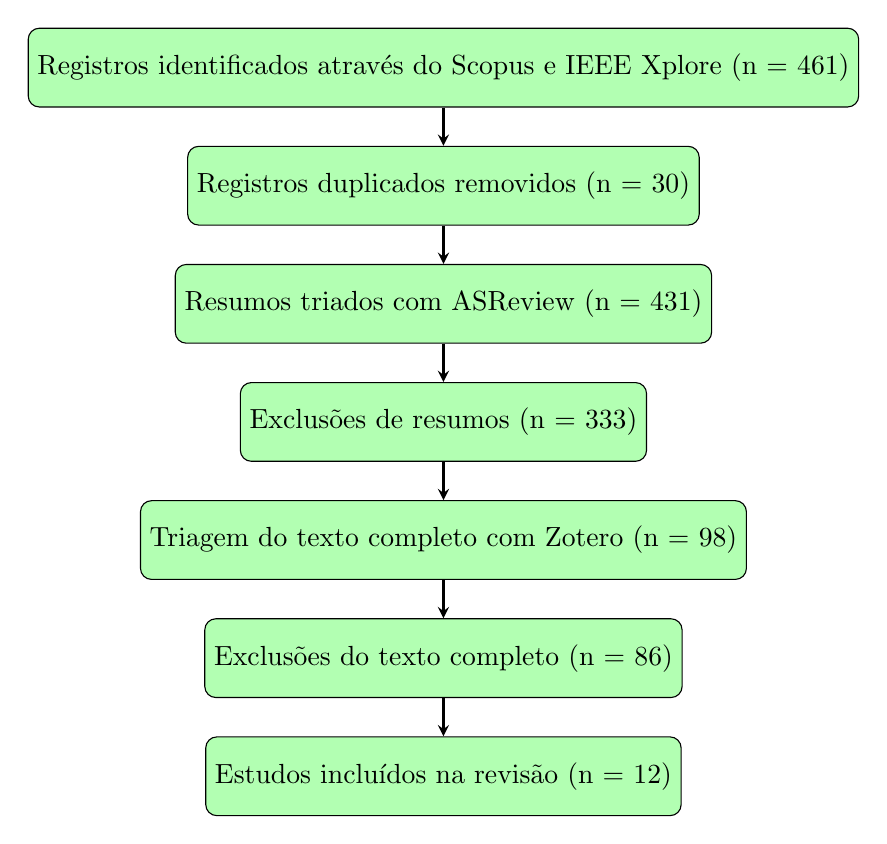
\begin{tikzpicture}[node distance=1.5cm] % Adjusted node distance for vertical spacing

% Define styles
\tikzstyle{process} = [rectangle, rounded corners, minimum width=2cm, minimum height=1cm, text centered, draw=black, fill=green!30]
\tikzstyle{arrow} = [thick,->,>=stealth]

% Nodes
\node (id) [process] {Registros identificados através do Scopus e IEEE Xplore (n = 461)};
\node (duplicates) [process, below of=id] {Registros duplicados removidos (n = 30)};
\node (screen1) [process, below of=duplicates] {Resumos triados com ASReview (n = 431)};
\node (exclude1) [process, below of=screen1] {Exclusões de resumos (n = 333)};
\node (screen2) [process, below of=exclude1] {Triagem do texto completo com Zotero (n = 98)};
\node (exclude2) [process, below of=screen2] {Exclusões do texto completo (n = 86)};
\node (include) [process, below of=exclude2] {Estudos incluídos na revisão (n = 12)};
% Arrows
\draw [arrow] (id) -- (duplicates);
\draw [arrow] (duplicates) -- (screen1);
\draw [arrow] (screen1) -- (exclude1);
\draw [arrow] (exclude1) -- (screen2);
\draw [arrow] (screen2) -- (exclude2);
\draw [arrow] (exclude2) -- (include);

\end{tikzpicture}
\caption{Fluxograma PRISMA ilustrando o processo de revisão sistemática}
\label{fig:prisma}
\end{figure}

\section{Resultados}
Os artigos selecionados destacam coletivamente o papel transformador das técnicas de Aprendizado por Reforço (RL) e Aprendizado Profundo (DL) no avanço das capacidades dos sistemas de enxame de VANTs. Por fim a tabela \ref{tab:swarm_summary} resume as informações dos trabalhos considerados.
\clearpage


%Tabela desajustada, arrumar
%\subsection{Resumo dos Trabalhos}
\begin{table*}[p]
\centering
\caption{Resumo dos trabalhos considerados pela revisão}
\renewcommand{\arraystretch}{1} % Adjust row height for vertical spreading
\setlength{\tabcolsep}{4pt} % Adjust column spacing
\resizebox{1\textwidth}{!}{
\begin{tabular}{|p{6cm}|p{4cm}|p{3cm}|p{3cm}|}
\hline
\textbf{Contribuição} & \textbf{Algoritmos} & \textbf{Arquitetura} & \textbf{Tarefa} \\ \hline
Dynamic formation control using DRL under operational uncertainty \cite{ID1}. & Proximal Policy Optimization (PPO), Deep Deterministic Policy Gradient (DDPG) & Centralized & Formation control, collision avoidance \\ \hline
Multi-agent PPO for combat UAV decision-making with reduced oscillation and enhanced stability \cite{ID2}. & Multi-Agent PPO & Centralized & Maneuvering decision-making \\ \hline
Distributed area coverage using FDSAC with centralized training and decentralized execution \cite{ID3}. & Fully Decentralized Soft Actor-Critic (FDSAC) & Decentralized & Dynamic area coverage \\ \hline
Multi-agent DRL for coverage-aware task allocation combining UAV and human collaboration \cite{ID4}. & Multi-Agent Actor-Critic (MAAC) & Decentralized & Task allocation, coverage optimization \\ \hline
Multi-drone shepherding for flock management using MTDDPG \cite{ID5}. & Multi-Task Deep Deterministic Policy Gradient (MTDDPG) & Decentralized & Shepherding, collision avoidance \\ \hline
MARL with adversarial randomization for robustness in dynamic environments \cite{ID6}. & Adversarial Domain Randomization with PPO & Decentralized & Dynamic task allocation, collision avoidance \\ \hline
Two-stage DRL for efficient target tracking with expert-guided exploration \cite{ID7}. & Double Deep Q-Network (DDQN), Expert-Guided Exploration & Decentralized & Target tracking \\ \hline
CBC-TP Net for UAV pursuit-evasion games in complex urban settings \cite{ID8}. & Cross-Boundary Cooperative Task-Planning Net (CBC-TP Net) & Decentralized & Pursuit-evasion \\ \hline
Vision-based formation control using YOLOv7 and DeepSORT in GNSS-denied environments \cite{ID9}. & YOLOv7, DeepSORT & Hybrid Hierarchical & Formation control \\ \hline
PPO with RNN layers for path planning in partially observable environments \cite{ID10}. & PPO with Recurrent Neural Network (RNN) layers & Decentralized & Path planning, collision avoidance \\ \hline
IPBO framework for multitarget tracking using island-based decentralized policy optimization \cite{ID11}. & Island Policy-Based Optimization (IPBO) & Decentralized & Multitarget tracking \\ \hline
Belief-policy interrelation framework using GAIL for coordination in heterogeneous swarms \cite{ID12}. & Generative Adversarial Imitation Learning (GAIL) & Decentralized & Coordination, formation control \\ \hline
\end{tabular}
}
\label{tab:swarm_summary}
\end{table*}




\clearpage



\subsection{Aprimoramento na Execução de Tarefas}
\subsubsection{Controle Dinâmico de Formação}
Vários artigos, incluindo \cite{ID1}, demonstram a integração de algoritmos de RL e DL para permitir que enxames de VANTs mantenham formações sinérgicas em ambientes incertos. Por exemplo, o framework P-DRL em \cite{ID1}, utilizando algoritmos como A3C e DQN, aborda a incerteza operacional ao dividir o problema de controle em subproblemas mais simples, reduzindo significativamente a complexidade computacional, enquanto mantém a capacidade de resposta em tempo real. No entanto, limitações na prevenção de colisões indicam que melhorias adicionais na interação entre múltiplos agentes são necessárias.

\subsubsection{Manobras e Rastreamento de Múltiplos Alvos}
Os artigos \cite{ID2} e \cite{ID11} enfrentam os desafios da tomada de decisão cooperativa e do rastreamento de múltiplos alvos em ambientes 3D dinâmicos. Utilizando métodos avançados de MARL, como MP3O e frameworks otimizados por recompensa, esses trabalhos alcançam melhorias notáveis na eficiência da tomada de decisão e na versatilidade do enxame. Além disso, o conceito de enxame dinâmico em \cite{ID11} oferece soluções inovadoras para particionamento e reagrupamento de VANTs com base na distribuição de alvos, aumentando a flexibilidade operacional.

\subsubsection{Alocação de Tarefas e Cobertura de Área}
A alocação de tarefas e a cobertura de área emergem como áreas de foco críticas em \cite{ID4} e \cite{ID3}. Os algoritmos baseados em DRL propostos distribuem de forma eficiente as tarefas de sensoriamento e ajustam dinamicamente os pontos de cobertura. Por exemplo, o método de alocação de tarefas Pareto-ótimo em \cite{ID4} combina a colaboração entre VANTs e humanos, enfatizando aplicações no mundo real, como cidades inteligentes e serviços públicos. Esses estudos ressaltam o potencial das técnicas de DL na otimização do desempenho das tarefas, ao mesmo tempo em que lidam com restrições como comunicação e poder computacional.

\subsubsection{Prevenção de Colisões e Navegação}
Técnicas como as descritas em \cite{ID7} e \cite{ID11} priorizam a navegação segura e a prevenção de obstáculos por meio de mecanismos avançados de recompensa e frameworks de treinamento com RL. A abordagem DRL em duas etapas apresentada em \cite{ID7}, incorporando experiência de especialistas, melhora a velocidade de convergência e a capacidade de generalização em ambientes dinâmicos. Isso reduz os custos de treinamento, garantindo uma navegação confiável para múltiplos agentes.


\subsection{Melhorias de Desempenho e Trade-Offs}
\subsubsection{Escalabilidade}
A escalabilidade, um desafio crítico em sistemas de enxame de VANTs, foi abordada de forma eficaz em diversos estudos. Por exemplo, o framework P-DRL em \cite{ID1} demonstrou controle de formação em tempo real para enxames compostos por 10–20 VANTs, ampliando significativamente a escalabilidade da coordenação multiagente. Da mesma forma, \cite{ID11} introduziu um conceito de enxame dinâmico que permitiu a partição e reagrupamento de grupos de VANTs de forma adaptativa, garantindo flexibilidade para atender às mudanças nos requisitos das tarefas. Essas abordagens ressaltam o potencial dos métodos de RL na expansão das operações do enxame sem comprometer o desempenho, embora frequentemente exijam recursos computacionais substanciais durante o treinamento.

\subsubsection{Tempo de Execução}
A redução do tempo de execução para tarefas como planejamento dinâmico de trajetória e controle de formação é essencial para aplicações em tempo real. Estudos como \cite{ID5} utilizaram aprendizado por reforço profundo multitarefa (MT-DDPG) para acelerar a conclusão de operações de pastoreio. Da mesma forma, \cite{ID9} empregou modelos leves de DL, como o YOLOv7, para realizar controle de formação baseado em visão em tempo real, demonstrando tempos de execução adequados para processamento embarcado. No entanto, essas melhorias aumentam a complexidade algorítmica e exigem treinamento intensivo em recursos computacionais.

\subsubsection{Taxa de Sucesso}
O aprimoramento da taxa de sucesso em tarefas do enxame, como prevenção de colisões e alocação dinâmica de tarefas, foi um foco central. Por exemplo, \cite{ID2} relatou maior estabilidade e eficiência na tomada de decisão cooperativa utilizando o algoritmo MP3O, melhorando as taxas de sucesso em manobras de combate aéreo. Além disso, \cite{ID7} demonstrou que o pré-treinamento de agentes com dados especializados levou a uma convergência mais rápida e a resultados de rastreamento mais confiáveis, especialmente em ambientes com obstáculos. No entanto, esses sucessos geralmente dependem de um design cuidadoso das funções de recompensa e otimizações específicas do domínio, o que pode limitar a generalização dos métodos.

\subsubsection{Resiliência}
A resiliência a incertezas ambientais e falhas do sistema foi destacada em estudos que empregam técnicas de randomização de domínio. \cite{ID6} propôs a randomização adversarial de domínio para melhorar a robustez das políticas MARL na transição de simulação para realidade, garantindo desempenho consistente em diversos cenários operacionais. Da mesma forma, \cite{ID8} introduziu um framework de perseguição e evasão que manteve o sucesso da missão mesmo quando alguns VANTs do enxame foram comprometidos. Embora esses métodos aumentem a resiliência, geralmente exigem alto custo computacional e ambientes de simulação extensivos para um treinamento eficaz.

\subsubsection{Trade-Offs}
\begin{itemize}
    \item \textbf{Demandas Computacionais}: Métodos como randomização adversarial de domínio \cite{ID6} e frameworks hierárquicos profundos \cite{ID8} exigem altos recursos computacionais, o que pode limitar sua implementação em sistemas de VANTs com restrições de hardware.
    \item \textbf{Complexidade do Treinamento}: Técnicas que enfatizam adaptabilidade e resiliência, como reconfiguração dinâmica de enxame \cite{ID11} ou DRL em duas etapas \cite{ID7}, frequentemente envolvem pipelines de treinamento complexos, demandando expertise significativa e tempo de desenvolvimento.
    \item \textbf{Implantação no Mundo Real}: Embora os resultados em simulação sejam promissores, métodos como P-DRL \cite{ID1} e MP3O \cite{ID2} enfrentam desafios na transição para aplicações reais devido a fatores como imprecisões nos sensores e restrições de comunicação.
\end{itemize}



\section{Discussão}
\subsection{Principais Descobertas}
Esta revisão sistemática explorou as contribuições das técnicas de Aprendizado por Reforço (RL) e Aprendizado Profundo (DL) para o avanço dos sistemas de enxame de VANTs, destacando seu potencial transformador na solução de desafios críticos. Nos artigos revisados, foram alcançadas melhorias significativas em escalabilidade, tempo de execução, taxa de sucesso e resiliência. As principais contribuições incluem:

\begin{itemize}
    \item \textbf{Controle Dinâmico de Formação}: Estudos como \cite{ID1} demonstraram frameworks capazes de realizar controle de formação em tempo real para enxames de VANTs de médio porte, reduzindo a complexidade computacional por meio de algoritmos avançados de RL, como A3C e DQN.
    \item \textbf{Tomada de Decisão Multiagente e Rastreamento}: Abordagens inovadoras, como MP3O (\cite{ID2}) e conceitos de enxame dinâmico (\cite{ID11}), aprimoraram significativamente a tomada de decisão cooperativa e o rastreamento de múltiplos alvos, melhorando a eficiência operacional e a adaptabilidade.
    \item \textbf{Alocação de Tarefas e Cobertura de Área}: Métodos como alocação de tarefas Pareto-ótima (\cite{ID4}) e cobertura baseada em FDSAC (\cite{ID3}) apresentaram técnicas eficazes para equilibrar a distribuição da carga de trabalho e otimizar a eficiência do sensoriamento, mesmo em ambientes com restrições de comunicação.
    \item \textbf{Prevenção de Colisões e Navegação}: Frameworks como os descritos em \cite{ID7} e \cite{ID6} forneceram soluções robustas para navegação em ambientes complexos, com avanços em modelagem de recompensas e randomização de domínio, garantindo operações livres de colisões e melhores transições entre simulação e realidade.
    \item \textbf{Validações em Ambientes Reais}: Alguns estudos (\cite{ID5}, \cite{ID9}) validaram seus métodos em cenários reais, demonstrando viabilidade prática e oferecendo uma base para melhorias futuras.
\end{itemize}

\subsection{Lacunas e Desafios Não Resolvidos}
Apesar desses avanços, diversas lacunas permanecem, apontando para oportunidades de pesquisa futura:
\begin{enumerate}
    \item \textbf{Escalabilidade para Enxames Maiores}: Embora muitos métodos tenham melhorado a coordenação em enxames de médio porte (por exemplo, 10–20 VANTs em \cite{ID1}), a escalabilidade para enxames maiores ainda é um desafio aberto. São necessários algoritmos eficientes que possam escalar sem um aumento proporcional na complexidade computacional.
    \item \textbf{Redução da Lacuna entre Simulação e Realidade}: Embora métodos de randomização de domínio (\cite{ID6}) tenham mostrado potencial, a tradução dos resultados simulados para operações no mundo real é limitada por ruído nos sensores, variabilidade ambiental e restrições do sistema. Melhorar a robustez em aplicações reais continua sendo essencial.
    \item \textbf{Eficiência Energética e Otimização de Recursos}: Embora alguns estudos tenham abordado o consumo de energia indiretamente, estratégias dedicadas para otimizar o uso energético em todo o enxame ainda são pouco exploradas.
    \item \textbf{Métricas Padronizadas e Benchmarking}: A ausência de métricas padronizadas entre os estudos (\cite{ID3}, \cite{ID4}) dificulta comparações diretas. O estabelecimento de um framework unificado de benchmarking facilitaria avaliações consistentes do desempenho dos enxames.
    \item \textbf{Integração de Sistemas Heterogêneos}: Estudos como \cite{ID12} introduziram esforços iniciais para a coordenação de enxames heterogêneos, mas são necessárias investigações mais aprofundadas sobre o equilíbrio das disparidades de recursos e a alocação de tarefas entre diferentes tipos de VANTs.
\end{enumerate}

\section{Comparação com Estado da Arte}
A tabela \ref{tab:marl_comparison} ilustra como o trabalho proposto se posiciona em relação aos trabalhos da revisão de literatura. Os critérios adotados na comparação foram:
\begin{itemize}
    \item Execução Descentralizada (DE): Verifica se a abordagem adotada pelo trabalho possibilita execução descentralizada pelos agentes, isto é, se o enxame não necessita de um nó central que envia os comandos para execução.
    
    \item Escalabilidade (Scalable): Verifica se a abordagem de controle do enxame permite a quantidade de agentes pode aumentar sem afetar o desempenho.
    
    \item Coordenação (Coord): Se há coordenação entre as ações dos agentes no ambiente que executam a missão.
    
    \item Espaço de Ação Contínuo (Cont): Verifica se o domínio do espaço de ações dos agente é contínuo ou discreto.
    
    \item Visão Computacional (Vision): Se a abordagem utiliza algum tipo de informação visual capturada pelos agentes em seu espaço de observações do algoritmo.
    
    \item Comunicação (Comm): Se há troca de informações entre os agentes através de algum meio de comunição.
    
    \item Missão Global (GM): Se a missão do enxame envolve tarefas complexas além das tarefas atividades comuns, como por exemplo: rastreamento de alvos, transporte de carga, cobertura de área e reconstrução 3D.
    
    \item Planejamento de Caminho (PP): Se o trabalho lida com a atividade de planejamento de trajetória.
    
    \item Prevenção de Colisões (CA): Se o trabalho aborda a atividade de prevenção de colisões.
    
    \item Controle de Formação (FC): Se o trabalho aborda a atividade do controle de formação do enxame.
\end{itemize}

\paragraph{Ajustar tabela para o CAP 5 secao de comparacao com SOTA}
\begin{table}[h]
\centering
\caption{Quadro comparativo da proposta com estado da arte.}
\label{tab:marl_comparison}
\begin{adjustbox}{width=\textwidth}
\begin{tabular}{ccccccccccc}
\toprule
  Trabalho &DE&Scalable&Coord&Cont&Vision&Comm&GM&PP&CA&FC \\
  
\midrule
  \cite{ID1} &  \xmark & \cmark & \cmark & \cmark & \xmark & \cmark & \xmark & \cmark & \cmark &\cmark  \\
  \cite{ID2} &  \cmark & \xmark & \xmark & \cmark & \xmark & \xmark & \cmark & \cmark & \xmark &\xmark \\
  \cite{ID3} &  \cmark & - & \xmark & \xmark & \xmark & \cmark & \cmark & \xmark & \cmark & \xmark  \\
  \cite{ID4} &  \cmark & \xmark & \cmark & \xmark & \xmark & \xmark & \cmark & \cmark & \cmark & \xmark\\
  \cite{ID5} &  \cmark & \xmark & \cmark & \cmark & \xmark & \xmark & \cmark & \cmark & \xmark & \cmark \\
  \cite{ID6} &  \cmark & \xmark & \cmark & \cmark & \cmark & - & \cmark & \cmark & \xmark & \cmark \\
  \cite{ID7} &  \cmark & \xmark & \cmark & \cmark & \cmark & \xmark & \cmark & \cmark & \cmark & \xmark \\
  \cite{ID8} &  \cmark & \xmark & \cmark & \cmark & \xmark & \cmark & \cmark & \cmark & \cmark & \xmark \\
  \cite{ID9} &  \xmark & \xmark & \cmark & \cmark & \cmark & \cmark & \xmark & \xmark & \xmark & \cmark \\
  \cite{ID10} &  \cmark & \xmark & \xmark & \cmark & \xmark & \cmark & \xmark & \cmark & \cmark & \xmark \\
  \cite{ID11} &  \cmark & \cmark & \cmark & \xmark & \xmark & \xmark & \cmark & \cmark & \cmark & \cmark \\
  \cite{ID12} &  \cmark & \xmark & \cmark & \cmark & \xmark & \xmark & \xmark & \xmark & \xmark & \cmark  \\
  Proposta &  \cmark & \cmark & \cmark & - & \cmark & \cmark & \cmark & \cmark & \cmark &\cmark  \\
\bottomrule
\end{tabular}
\end{adjustbox}
\end{table}

% \section{Atualização do Estado da Arte Assistida por Ferramentas de IA}

% Com o objetivo de atualizar o estado da arte e incorporar trabalhos recentes publicados após a condução da revisão sistemática formal, foi realizada uma etapa complementar de busca bibliográfica assistida por ferramentas de inteligência artificial. Nesta etapa, utilizou-se um mecanismo de busca baseado em modelos de linguagem de grande porte, configurado para consultar bases acadêmicas consolidadas, como IEEE Xplore, Elsevier e arXiv.

% As consultas foram estruturadas a partir das mesmas questões de pesquisa (RQ1–RQ6) e dos termos definidos no framework PICO, garantindo consistência metodológica com a revisão sistemática original. Os resultados retornados foram submetidos a uma curadoria manual rigorosa, incluindo leitura de títulos, resumos e, quando pertinente, do texto completo, bem como aplicação dos mesmos critérios de inclusão e exclusão previamente definidos.

% É importante destacar que a ferramenta de IA foi utilizada exclusivamente como um meio de apoio à identificação de estudos relevantes, não substituindo o julgamento crítico do pesquisador nem os procedimentos formais de seleção e análise dos trabalhos incluídos nesta dissertação.


\chapter{Desenvolvimento do Trabalho}
\label{cap:desenvolvimento}

Este capítulo descreve o desenvolvimento do trabalho proposto, abordando a modelagem do problema de navegação cooperativa de enxames de veículos aéreos não tripulados, os ambientes de simulação adotados, a definição das tarefas, dos espaços de estados e ações, das funções de recompensa e das estratégias de treinamento empregadas no contexto de aprendizado por reforço multiagente.

A abordagem investigada tem como objetivo o aprendizado de políticas de controle de alto nível para coordenação de enxames de VANTs, não atuando diretamente no controle de baixo nível dos veículos, mas na tomada de decisões estratégicas a partir de observações do ambiente. Essa estrutura é ilustrada de forma esquemática na Figura~\ref{fig:framework_idea}, que apresenta o loop de aprendizado por reforço entre os agentes, o ambiente de simulação e as Máquinas de Recompensa, destacando o paradigma de treinamento centralizado com execução descentralizada (\textit{Centralized Training with Decentralized Execution} -- CTDE).

Inicialmente, os experimentos foram conduzidos no simulador AirSim, em função de sua integração com controladores de voo amplamente utilizados, como ArduPilot e PX4, permitindo a validação conceitual da modelagem do problema e da formulação da função de recompensa em um ambiente tridimensional realista. No entanto, devido às limitações computacionais associadas à execução de algoritmos de aprendizado por reforço multiagente e à necessidade de maior escalabilidade experimental, optou-se pela adoção do simulador IsaacSim, em conjunto com o framework IsaacLab, como plataforma principal para o treinamento final dos modelos e a obtenção dos resultados apresentados neste trabalho.

Ressalta-se que a utilização prévia do AirSim desempenhou um papel fundamental na fase inicial da pesquisa, contribuindo para a compreensão do problema, a validação das hipóteses propostas e o refinamento da metodologia experimental posteriormente aplicada no IsaacSim.

\begin{figure}
    \centering
    \includegraphics[width=0.8\textwidth]{fig/improved_rm_marl_overview_framework.jpeg}
    \caption{Esquema geral do framework de aprendizado por reforço multiagente para controle de enxames de VANTs desenvolvido neste trabalho.}
    \label{fig:framework_idea}
\end{figure}

% =========================================================
\section{Modelagem do Problema}
\label{sec:modelagem_problema}

Esta seção apresenta a modelagem formal do problema de navegação cooperativa de enxames de VANTs, contemplando os ambientes de simulação adotados, a definição das tarefas, os espaços de estados e ações, e as funções de recompensa utilizadas no processo de aprendizado.
% TODO  - Fazer considerções gerais na modelagem formal do problema.
% Considerações: Discorrer sobre o objetivo da modelagem tentar representar um enxame de drones descentralizados. ou seja
% Cada drone deve tomar suas próprias decisões baseadas em suas observações locais e comunicação limitada com outros drones.
% Discutir sobre as limitações de sensores, gps, comunicação e ruídos nas leituras.
% ---------------------------------------------------------
\subsection{Ambientes de Simulação}
\label{subsec:ambientes_simulacao}

%A utilização de ambientes de simulação fidedignos e escaláveis é um fator determinante no desenvolvimento e validação de algoritmos de aprendizado por reforço aplicados ao controle de enxames de veículos aéreos não tripulados. Neste trabalho, dois simuladores foram empregados ao longo das diferentes etapas de desenvolvimento: o AirSim e o IsaacSim. Cada um desses ambientes apresenta características específicas, tendo sido concebidos com finalidades distintas, o que impacta diretamente sua adequação a diferentes fases do processo experimental.

O AirSim é um simulador de código aberto desenvolvido inicialmente pela Microsoft Research, apresentado por \citeonline{shah2018airsim}, com o objetivo de apoiar pesquisas em veículos autônomos, incluindo carros e VANTs. Construído sobre o motor gráfico Unreal Engine, o AirSim oferece ambientes tridimensionais de alta fidelidade visual, suporte a sensores realistas — como câmeras RGB, profundidade, sensores de distância e IMU — e integração direta com controladores de voo amplamente utilizados, como ArduPilot e PX4. Essa arquitetura permite que o simulador funcione como uma camada de abstração entre algoritmos de alto nível e controladores de baixo nível, aproximando o comportamento do sistema simulado daquele observado em operações reais.

Entre os principais pontos fortes do AirSim destacam-se sua especialização em aplicações com VANTs, a facilidade de configuração de sensores e cenários personalizados, bem como a possibilidade de realizar testes de voo autônomo baseados em scripts e missões pré-programadas. Por outro lado, o simulador apresenta limitações relacionadas ao desempenho computacional e à escalabilidade, especialmente em cenários que envolvem múltiplos agentes e demandam a execução paralela de diversos ambientes, o que pode comprometer a eficiência do treinamento de algoritmos de aprendizado por reforço multiagente.

O IsaacSim, por sua vez, é um simulador desenvolvido pela NVIDIA, fundamentado na plataforma Omniverse e apresentado como uma solução voltada à simulação robótica de alto desempenho~\cite{makoviychuk2021isaac}. Diferentemente do AirSim, o IsaacSim foi projetado desde sua concepção para oferecer escalabilidade, paralelização massiva e integração nativa com bibliotecas de aprendizado profundo. O simulador utiliza tecnologias como USD (Universal Scene Description), PhysX para simulação física e RTX para renderização acelerada por hardware, possibilitando a execução simultânea de centenas ou milhares de ambientes em GPU.

Os principais pontos fortes do IsaacSim incluem seu elevado desempenho computacional, suporte robusto à paralelização de ambientes, fidelidade física e integração direta com frameworks de aprendizado por reforço, como o IsaacLab. Essas características tornam o simulador particularmente adequado para o treinamento intensivo de políticas de controle baseadas em aprendizado por reforço, especialmente em contextos multiagentes. Em contrapartida, o IsaacSim apresenta uma curva de aprendizado mais acentuada e menor especialização nativa em aplicações aeronáuticas quando comparado ao AirSim, exigindo maior esforço na modelagem de dinâmicas específicas de VANTs.

A Figura~\ref{fig:formacao_v_airsim} ilustra um cenário de enxame de VANTs em formação em V modelado no ambiente AirSim, enquanto a Figura~\ref{fig:formacao_v_isaacsim} apresenta uma configuração equivalente implementada no IsaacSim.

\begin{figure}[htbp]
    \centering
    \includegraphics[width=0.8\textwidth]{fig/swarm_airsim.png}
    \caption{Enxame em formação em V no ambiente AirSim.}
    \label{fig:formacao_v_airsim}
\end{figure}

\begin{figure}[htbp]
    \centering
    \includegraphics[width=0.8\textwidth]{fig/isaac-sim-env.png}
    \caption{Enxame em formação em V no ambiente IsaacSim.}
    \label{fig:formacao_v_isaacsim}
\end{figure}

No que se refere à integração com bibliotecas de aprendizado por reforço, ambos os simuladores oferecem suporte a diferentes níveis de abstração. O AirSim disponibiliza APIs em Python que permitem sua integração com frameworks como Gymnasium, Stable-Baselines e PyTorch, embora essa integração exija, em geral, a implementação manual de wrappers para adaptação ao paradigma de ambientes do tipo Markov Decision Process (MDP). Essa característica torna o AirSim mais flexível, porém menos otimizado para treinamentos em larga escala.

O IsaacSim, por outro lado, fornece integração nativa com o ecossistema de aprendizado por reforço da NVIDIA por meio do IsaacLab, que implementa interfaces compatíveis com o Gymnasium e suporta diretamente bibliotecas como PyTorch. Essa integração facilita a definição de ambientes vetorizados, o gerenciamento de observações e recompensas em larga escala, bem como a implementação de algoritmos de aprendizado por reforço multiagente de forma eficiente e modular. Em razão dessas características, o IsaacSim foi adotado como a plataforma principal para o treinamento final dos modelos e a avaliação quantitativa dos resultados apresentados neste trabalho.

% ---------------------------------------------------------
\subsection{Especificação das Tarefas dos Agentes}
\label{subsec:especificacao_tarefas}

A tarefa especificada para os agentes do enxame consistiu na navegação cooperativa em formação em V com desvio de obstáculos, em um ambiente tridimensional. O objetivo principal foi fazer com que os agentes aprendessem a se deslocar de uma posição inicial até uma posição final, mantendo a formação predefinida, evitando colisões com obstáculos estáticos e preservando uma distância segura entre si durante toda a execução da missão.

De modo geral, em ambos os simuladores, o cenário foi modelado de forma que múltiplos obstáculos fossem posicionados entre a posição inicial do enxame e a posição final a ser alcançada. A cada reinicialização do ambiente, tanto a posição inicial dos agentes quanto a posição de destino eram alteradas de forma aleatória, garantindo diversidade nos episódios de treinamento e forçando os agentes a aprenderem estratégias generalizáveis de navegação e desvio de obstáculos.

Além do desvio de obstáculos, a tarefa impôs restrições adicionais relacionadas à coesão do enxame. Os agentes deveriam manter uma distância segura entre si, evitando tanto colisões quanto uma dispersão excessiva da formação, de modo a preservar o comportamento coletivo característico de uma navegação em formação em V.
%**Melhorias
%TODO -- Adicionar informações sobre os termos, métricas e condições de término dos episódios em cada simulador.
% Explicar oque signigica um step, episodio, etc.para que o leitor compreenda melhor as condições na proxima subseção.
\subsubsection{Ambiente AirSim}

No ambiente AirSim, a tarefa foi modelada considerando o uso de controladores de voo de baixo nível, como ArduPilot e PX4, fornecidos pelo próprio simulador. Dessa forma, a política de aprendizado por reforço atuou em um nível de abstração mais elevado, sendo responsável apenas pela coordenação dos comandos enviados aos controladores de voo, sem a necessidade de aprender diretamente a estabilização do voo.

Os obstáculos presentes nesse ambiente foram modelados como cilindros em forma de pilares, distribuídos horizontalmente de modo a bloquear o sentido principal de navegação do enxame. Essa configuração exigiu que os agentes realizassem manobras de desvio enquanto mantinham a formação durante o deslocamento.

\begin{figure}[htbp]
    \centering
    \includegraphics[width=0.8\textwidth]{fig/task_obstacles_airsim.png}
    \caption{Ambiente de obstáculos para navegação em formação de enxame no AirSim.}
    \label{fig:airsim_obstaculos}
\end{figure}

O término de um episódio no AirSim ocorreu com base em um conjunto de condições relacionadas ao sucesso da missão, à segurança da formação e à limitação do tempo de execução. Essas condições estão resumidas na Tabela~\ref{tab:termino_airsim}.

\begin{table}[htbp]
\centering
\caption{Condições de término e reinicialização de episódios no AirSim.}
\label{tab:termino_airsim}
\begin{tabular}{ll}
\hline
\textbf{Condição} & \textbf{Descrição} \\
\hline
Dispersão do enxame & Distância média entre agentes maior que três vezes a distância inicial \\
Desvio excessivo do alvo & Distância ao objetivo maior que cinco vezes a distância inicial \\
Objetivo alcançado & Centroide do enxame a menos de 3 m da posição final \\
Limite de passos & Número máximo de steps do episódio (1000 steps) \\
\hline
\end{tabular}
\end{table}

A condição de dispersão do enxame foi utilizada para encerrar episódios nos quais os agentes se afastavam excessivamente da formação desejada, enquanto a condição de desvio do alvo evitou episódios longos que não apresentavam progressos significativos em direção ao objetivo. O sucesso da missão foi caracterizado pela aproximação do centroide do enxame à posição final desejada.

\subsubsection{Ambiente IsaacSim}

No ambiente IsaacSim, a tarefa foi modelada de forma distinta, uma vez que o simulador não fornece, de maneira nativa, controladores de voo equivalentes ao PX4 ou ArduPilot. Assim, os agentes precisaram aprender políticas de controle de nível mais baixo, incluindo aspectos relacionados à estabilização do voo, o que impactou diretamente as condições de término e reinicialização dos episódios.

Durante as iterações iniciais de treinamento, era comum que os agentes perdessem estabilidade e colidissem com o solo. Dessa forma, foi definida uma condição de reinicialização sempre que a altitude de um agente fosse inferior a um limite mínimo. De modo análogo, limites superiores de altitude e restrições espaciais do ambiente foram empregados para evitar comportamentos indesejados, como a saída da região válida de simulação.

As condições de término e reinicialização adotadas no IsaacSim estão resumidas na Tabela~\ref{tab:termino_isaacsim}.

\begin{table}[htbp]
\centering
\caption{Condições de término e reinicialização de episódios no IsaacSim.}
\label{tab:termino_isaacsim}
\begin{tabular}{ll}
\hline
\textbf{Condição} & \textbf{Descrição} \\
\hline
Altitude mínima & Altura do agente inferior ao limite mínimo permitido \\
Altitude máxima & Altura do agente superior ao limite máximo permitido \\
Fora dos limites & Agente fora dos limites espaciais do ambiente \\
Tempo máximo & Duração máxima do episódio excedida \\
\hline
\end{tabular}
\end{table}

Com o objetivo de facilitar o aprendizado de comportamentos complexos, foi adotada no IsaacSim uma estratégia de aprendizado curricular, na qual o treinamento foi dividido em cinco estágios progressivos. Cada estágio buscou simplificar o comportamento a ser aprendido, adicionando gradualmente novos desafios à tarefa.

\subsubsubsection{Estágios do Curriculum Learning}
%\label{subsubsec:estagios_curriculum}

O treinamento dos agentes no ambiente IsaacSim foi estruturado segundo uma estratégia de aprendizado curricular (\textit{Curriculum Learning}), na qual a tarefa global de navegação cooperativa em formação com desvio de obstáculos foi decomposta em cinco estágios progressivos. Cada estágio foi projetado para enfatizar um subconjunto específico de habilidades, permitindo que os agentes adquirissem comportamentos básicos antes de serem expostos a desafios mais complexos. A Figura~\ref{fig:curriculum_overview} apresenta uma visão geral dos cenários adotados em cada etapa do currículo.

No primeiro estágio, denominado \textit{Hover} (Figura~\ref{fig:curriculum_stage1}), os drones iniciam o episódio com suas posições organizadas em forma de grid no plano \(xy\). As posições finais apresentam variação mínima nas coordenadas \(x\) e \(y\), enquanto a coordenada \(z\) é definida dentro de um intervalo configurável para cada agente. Essa configuração tem como objetivo enfatizar o aprendizado do controle de altitude, induzindo os agentes a aumentarem sua altura com deslocamento mínimo no plano horizontal. As posições finais desejadas são indicadas visualmente pelos pontos verdes, reforçando que o principal comportamento esperado nesse estágio é a ascensão vertical e a estabilização do voo.

No segundo estágio, ilustrado na Figura~\ref{fig:curriculum_stage2}, a tarefa consiste na navegação ponto a ponto no plano \(xy\), sem a consideração de comportamentos de enxame. Cada drone é alocado em uma “camada” distinta do espaço tridimensional, caracterizada por uma altura \(z\) fixa, com um deslocamento \(\Delta z\) entre os agentes. As posições finais mantêm a mesma coordenada \(z\) da posição inicial, sendo indicadas pelos pontos verdes, enquanto as coordenadas \(x\) e \(y\) são transladadas. Essa configuração força cada agente a aprender a se movimentar no plano horizontal correspondente à sua camada, preservando a altitude constante, o que contribui para o refinamento das habilidades de navegação planar.

O terceiro estágio, apresentado na Figura~\ref{fig:curriculum_stage3}, introduz obstáculos estáticos posicionados entre a posição inicial e a posição objetivo de cada drone. Nesse cenário, o objetivo principal é enfatizar o comportamento de desvio de obstáculos, induzindo os agentes a realizarem trajetórias do tipo zig-zag para contornar as barreiras. Neste estágio, os agentes ainda não consideram restrições relacionadas à distância entre si nem à manutenção de formação, concentrando-se exclusivamente na adaptação da trajetória para evitar colisões com os obstáculos. As posições finais continuam sendo indicadas pelos pontos verdes.

No quarto estágio, ilustrado na Figura~\ref{fig:curriculum_stage4}, o comportamento de enxame passa a ser explicitamente considerado. Os agentes iniciam o episódio organizados em uma formação em V, e as posições finais são definidas por meio de translações e rotações aplicadas à configuração inicial da formação. Essa característica força os agentes a aprenderem a navegar cooperativamente, preservando a geometria da formação e evitando colisões entre si. Nesse cenário, o marcador visual em azul representa o centroide do enxame, enquanto as posições finais individuais dos agentes são indicadas pelos pontos amarelos.

Por fim, o quinto estágio, representado na Figura~\ref{fig:curriculum_stage5}, corresponde ao cenário mais complexo do currículo. Nesse estágio, são adicionados obstáculos entre a posição inicial do enxame e a posição final desejada. Diferentemente dos estágios anteriores, a posição objetivo é definida em relação ao centroide do enxame, indicado visualmente por um cubo verde posicionado após a região de obstáculos. Esse arranjo reforça a necessidade de os agentes considerarem simultaneamente múltiplos fatores, incluindo a distância entre si, a proximidade dos obstáculos e a navegação coordenada em direção à posição final coletiva.

\begin{figure}[H]
    \centering

    \begin{subfigure}{0.45\textwidth}
        \centering
        \includegraphics[width=\textwidth]{fig/stage1_example.png}
        \caption{Estágio 1: Hover.}
        \label{fig:curriculum_stage1}
    \end{subfigure}
    \hfill
    \begin{subfigure}{0.45\textwidth}
        \centering
        \includegraphics[width=\textwidth]{fig/stage2_example.png}
        \caption{Estágio 2: Navegação ponto a ponto em camadas de altitude.}
        \label{fig:curriculum_stage2}
    \end{subfigure}

    \vspace{0.5em}

    \begin{subfigure}{0.45\textwidth}
        \centering
        \includegraphics[width=\textwidth]{fig/stage3_example.png}
        \caption{Estágio 3: Navegação com desvio de obstáculos.}
        \label{fig:curriculum_stage3}
    \end{subfigure}
    \hfill
    \begin{subfigure}{0.45\textwidth}
        \centering
        \includegraphics[width=\textwidth]{fig/stage4_example.png}
        \caption{Estágio 4: Navegação cooperativa em formação em V.}
        \label{fig:curriculum_stage4}
    \end{subfigure}

    \vspace{0.5em}

    \begin{subfigure}{0.6\textwidth}
        \centering
        \includegraphics[width=\textwidth]{fig/stage5_example.png}
        \caption{Estágio 5: Navegação em formação com obstáculos.}
        \label{fig:curriculum_stage5}
    \end{subfigure}

    \caption{Visão geral dos estágios do aprendizado curricular adotado no IsaacSim.}
    \label{fig:curriculum_overview}
\end{figure}

Essa estratégia de aprendizado curricular permitiu uma progressão gradual da complexidade da tarefa, contribuindo para a estabilidade do treinamento e para a aquisição de comportamentos cooperativos cada vez mais sofisticados. Os impactos dessa abordagem sobre a eficiência do aprendizado e o desempenho final dos agentes serão analisados nas seções subsequentes de treinamento e resultados.


% ---------------------------------------------------------

\subsection{Espaço de Estados e Ações}
\label{subsec:espaco_estados_acoes}

A definição do espaço de estados (ou observações) e do espaço de ações constitui um dos elementos centrais na formulação de problemas de aprendizado por reforço, pois estabelece a interface entre a percepção do agente e sua capacidade de atuação no ambiente. No contexto deste trabalho, esses espaços foram projetados de modo a refletir informações que seriam, em princípio, acessíveis a um VANT real por meio de sensores embarcados e atuadores físicos, garantindo coerência entre a modelagem em simulação e uma possível aplicação em cenários reais.

Cada agente observa apenas informações locais e parciais do ambiente, caracterizando um problema de decisão sob observabilidade parcial. Em contrapartida, durante a fase de treinamento centralizado, informações adicionais de caráter global podem ser exploradas pelo crítico, conforme o paradigma de \textit{Centralized Training with Decentralized Execution} (CTDE). Essa distinção permite que o aprendizado seja auxiliado por um ``oráculo'' durante o treinamento, enquanto a política aprendida permanece executável de forma descentralizada, utilizando exclusivamente observações locais.

\subsubsection{Espaço de Observação}

De forma geral, o vetor de observação de cada agente é composto por informações proprioceptivas, informações relativas à tarefa e percepções do ambiente. As informações proprioceptivas incluem estados cinemáticos do próprio agente, como posição, velocidade e orientação. As informações relativas à tarefa abrangem medidas associadas à posição objetivo, permitindo que o agente avalie seu progresso em relação à missão. Por fim, as percepções do ambiente são obtidas a partir de sensores simulados, como sensores de distância, raycasts ou câmeras, utilizados para detectar obstáculos e a presença de outros agentes no entorno.

No contexto multiagente, cada agente possui acesso apenas a observações locais de seus vizinhos mais próximos, como posições ou velocidades relativas, reforçando a natureza descentralizada do problema. Informações globais, como o estado completo do enxame ou o centroide global, são utilizadas exclusivamente pelo crítico durante o treinamento e não estão disponíveis para a política durante a execução.

A Figura~\ref{fig:obs_action_space} ilustra de forma conceitual o espaço de observação e o espaço de ações de um agente do enxame.

\begin{figure}[H]
    \centering
    \includegraphics[width=0.9\textwidth]{fig/uav_perception.jpeg}
    \caption{Ilustração conceitual do espaço de observação e do espaço de ações de um agente do enxame.}
    \label{fig:obs_action_space}
\end{figure}

\subsubsection{Espaço de Ações}

O espaço de ações adotado neste trabalho é contínuo, refletindo a natureza do controle de VANTs. As ações correspondem a comandos que influenciam diretamente a dinâmica do agente, podendo representar velocidades desejadas, acelerações, empuxos ou momentos, a depender do nível de abstração adotado pelo simulador. Essa modelagem permite a aplicação de algoritmos de aprendizado por reforço contínuo e a representação adequada de comportamentos de navegação e controle.

\subsubsection{Instanciação no Ambiente AirSim}

No ambiente AirSim, o espaço de observação de cada agente é multimodal, combinando informações visuais e vetoriais provenientes de diferentes sensores simulados. Para um agente $i$ no instante $t$, a observação local é definida como:
\[
\mathbf{o}_i^t =
\big[
\mathbf{I}_i^t,
\mathbf{p}_i^t,
\boldsymbol{\theta}_i^t,
\mathbf{v}_i^t,
d_{i,g}^t,
d_{i,o}^t,
\mathbf{d}_{i,\mathcal{N}}^t
\big].
\]

Cada componente do vetor de observação possui significado físico e dimensionalidade bem definida, conforme descrito a seguir:

\begin{itemize}
    \item $\mathbf{I}_i^t \in \mathbb{R}^{64 \times 64 \times 1}$: imagem de profundidade capturada pelo agente $i$, utilizada para a percepção espacial do ambiente e detecção de obstáculos à frente do drone.
    
    \item $\mathbf{p}_i^t \in \mathbb{R}^{3}$: vetor de posição tridimensional do agente, expresso no referencial global do ambiente, representando as coordenadas $(x, y, z)$ em metros.
    
    \item $\boldsymbol{\theta}_i^t \in \mathbb{R}^{3}$: vetor de orientação do agente, composto pelos ângulos de guinada (\textit{yaw}), arfagem (\textit{pitch}) e rolagem (\textit{roll}), em radianos.
    
    \item $\mathbf{v}_i^t \in \mathbb{R}^{3}$: vetor de velocidade linear do agente, representando as componentes $(v_x, v_y, v_z)$ no espaço tridimensional, em metros por segundo.
    
    \item $d_{i,g}^t \in \mathbb{R}$: distância escalar entre o agente $i$ e a posição objetivo, medida em metros, utilizada para avaliar o progresso da navegação em direção ao destino.
    
    \item $d_{i,o}^t \in \mathbb{R}$: distância frontal ao obstáculo mais próximo detectado pelo agente, medida em metros, fornecida por sensores de distância simulados.
    
    \item $\mathbf{d}_{i,\mathcal{N}}^t \in \mathbb{R}^{N \times N}$: matriz de distâncias interagentes, onde cada elemento representa a distância euclidiana, em metros, entre pares de agentes do enxame.
\end{itemize}

Durante o treinamento centralizado, o crítico tem acesso a uma observação global contendo informações completas do enxame, incluindo estados e relações espaciais entre todos os agentes. Essas informações não estão disponíveis durante a execução descentralizada das políticas, caracterizando explicitamente um problema sob observabilidade parcial, conforme o paradigma de \textit{Centralized Training with Decentralized Execution} (CTDE).

O espaço de ações no ambiente AirSim é contínuo e definido, para cada agente $i$ no instante $t$, como:
\[
\mathbf{a}_i^t =
\begin{bmatrix}
v_{x,i}^t &
v_{y,i}^t &
v_{z,i}^t &
\dot{\psi}_i^t
\end{bmatrix}
\in [-1,1]^4,
\]
onde $v_{x,i}^t$, $v_{y,i}^t$ e $v_{z,i}^t$ representam comandos normalizados de velocidade linear ao longo dos eixos cartesianos, e $\dot{\psi}_i^t$ corresponde ao comando normalizado de taxa de guinada (\textit{yaw rate}). Esses comandos são interpretados por um controlador de voo embarcado, como PX4 ou ArduPilot, responsável pela estabilização e pelo controle dinâmico do VANT. Dessa forma, a política de aprendizado por reforço atua em um nível de abstração elevado, focando em decisões de navegação e deslocamento, enquanto o controle de baixo nível é delegado ao controlador interno do simulador.


\subsubsection{Instanciação no Ambiente IsaacSim}

No ambiente IsaacSim, o espaço de observação adotado para cada agente é definido como um vetor contínuo de dimensão fixa. Diferentemente do AirSim, não são utilizadas observações visuais, sendo o estado completamente descrito por informações vetoriais diretamente relacionadas à dinâmica do VANT, à tarefa e às interações locais com o ambiente e com outros agentes. Para um agente $i$ no instante $t$, a observação individual é dada por:
\[
\mathbf{o}_i^t \in \mathbb{R}^{23}.
\]

Esse vetor é obtido pela concatenação dos seguintes componentes, cada um com significado físico e dimensionalidade bem definida:
\[
\mathbf{o}_i^t =
\big[
\mathbf{v}_i^t,
\boldsymbol{\omega}_i^t,
\mathbf{g}_i^t,
\mathbf{p}_{i,g}^t,
d_{i,o}^t,
\Delta \mathbf{v}_{i,\mathcal{N}}^t,
\Delta \mathbf{p}_{i,\mathcal{N}}^t,
\mathbf{q}_i^t
\big].
\]

A descrição detalhada de cada termo é apresentada a seguir:

\begin{itemize}
    \item $\mathbf{v}_i^t \in \mathbb{R}^{3}$: vetor de velocidade linear do agente, expresso no referencial do corpo, representando as componentes $(v_x, v_y, v_z)$ em metros por segundo.
    
    \item $\boldsymbol{\omega}_i^t \in \mathbb{R}^{3}$: vetor de velocidades angulares do agente, correspondente às taxas de rolagem, arfagem e guinada $(\omega_x, \omega_y, \omega_z)$, em radianos por segundo.
    
    \item $\mathbf{g}_i^t \in \mathbb{R}^{3}$: vetor da gravidade projetado no referencial do corpo do drone, utilizado como referência para orientação e estabilização do voo.
    
    \item $\mathbf{p}_{i,g}^t \in \mathbb{R}^{3}$: vetor posição relativa entre o agente $i$ e seu objetivo individual, expresso no referencial do corpo, indicando a direção e magnitude do deslocamento necessário para que o agente avance em direção à sua meta designada.
    
    \item $d_{i,o}^t \in \mathbb{R}$: distância escalar ao obstáculo mais próximo, medida em metros, obtida a partir de sensores de distância simulados.
    
    \item $\Delta \mathbf{v}_{i,\mathcal{N}}^t \in \mathbb{R}^{3}$: vetor de velocidade relativa entre o agente $i$ e seu vizinho mais próximo, utilizado para modelar interações locais e auxiliar na prevenção de colisões.
    
    \item $\Delta \mathbf{p}_{i,\mathcal{N}}^t \in \mathbb{R}^{3}$: vetor de posição relativa entre o agente $i$ e seu vizinho mais próximo, expresso no referencial do corpo, permitindo que o agente avalie sua proximidade em relação aos demais membros do enxame.
    
    \item $\mathbf{q}_i^t \in \{0,1\}^{4}$: vetor \textit{one-hot} que representa o estado corrente da Reward Machine associada ao agente, codificando o progresso da tarefa dentro da estratégia de aprendizado curricular.
\end{itemize}

Durante o treinamento centralizado, o crítico tem acesso ao estado global do sistema, definido como a concatenação direta das observações individuais de todos os agentes:
\[
\mathbf{s}^t =
\big[
\mathbf{o}_1^t,
\mathbf{o}_2^t,
\dots,
\mathbf{o}_N^t
\big]
\in \mathbb{R}^{23N}.
\]
Esse estado global não está disponível durante a execução descentralizada das políticas, caracterizando explicitamente um problema sob observabilidade parcial e mantendo consistência com o paradigma de \textit{Centralized Training with Decentralized Execution} (CTDE). Ressalta-se que informações relacionadas ao centroide do enxame são utilizadas apenas em condições de término dos episódios e não fazem parte do espaço de observação dos agentes.


No ambiente IsaacSim, o espaço de ações também é contínuo e definido, para cada agente $i$ no instante $t$, como:
\[
\mathbf{a}_i^t =
\begin{bmatrix}
T_i^t &
M_{x,i}^t &
M_{y,i}^t &
M_{z,i}^t
\end{bmatrix}
\in [-1,1]^4,
\]
onde $T_i^t$ representa o comando normalizado de empuxo total aplicado ao VANT, e $M_{x,i}^t$, $M_{y,i}^t$ e $M_{z,i}^t$ correspondem aos momentos normalizados aplicados em torno dos eixos de rolagem, arfagem e guinada, respectivamente. Esses comandos são aplicados diretamente ao modelo dinâmico do VANT no simulador, não havendo uma camada intermediária de controle baseada em controladores de voo embarcados. Consequentemente, a política aprendida é responsável não apenas pelo comportamento de navegação, mas também pela estabilização e pelo controle dinâmico do agente.




\subsubsection{Síntese Comparativa}

A Figura~\ref{fig:action_space_comparison} apresenta uma visão comparativa dos fluxos de controle e dos níveis de abstração associados aos espaços de ações adotados nos ambientes AirSim e IsaacSim. Observa-se que, embora ambos utilizem espaços de ações contínuos de mesma dimensionalidade, o significado físico dos comandos e a responsabilidade atribuída à política de aprendizado diferem substancialmente entre os simuladores.

Em particular, o AirSim favorece uma modelagem baseada em observações multimodais e ações de alto nível, suportadas por controladores de voo embarcados, enquanto o IsaacSim adota uma representação mais compacta do espaço de observação e ações aplicadas diretamente à dinâmica do agente. Essas diferenças motivaram escolhas distintas de arquiteturas neurais e estratégias de treinamento, conforme discutido nas seções subsequentes, sem comprometer a coerência conceitual da tarefa de navegação cooperativa em formação.

\begin{figure}[H]
\centering
\begin{tikzpicture}[
    node distance=1.3cm,
    every node/.style={
        draw,
        align=center,
        minimum width=3.0cm,
        minimum height=0.8cm,
        font=\footnotesize
    },
    arrow/.style={->, thin}
]

% ======================
% AirSim column
% ======================
\node[draw=none, font=\footnotesize\bfseries] (airsim_title) {AirSim};
\node (airsim_policy) [below of=airsim_title] {Política RL};
\node (airsim_action) [below of=airsim_policy] {$[v_x,\; v_y,\; v_z,\; \dot{\psi}]$};
\node (airsim_ctrl) [below of=airsim_action] {Controlador de Voo};
\node (airsim_dyn) [below of=airsim_ctrl] {Dinâmica};
\node (airsim_env) [below of=airsim_dyn] {Ambiente};

\draw[arrow] (airsim_policy) -- (airsim_action);
\draw[arrow] (airsim_action) -- (airsim_ctrl);
\draw[arrow] (airsim_ctrl) -- (airsim_dyn);
\draw[arrow] (airsim_dyn) -- (airsim_env);

% ======================
% IsaacSim column
% ======================
\node[draw=none, font=\footnotesize\bfseries, right=4.6cm of airsim_title] (isaac_title) {IsaacSim};
\node (isaac_policy) [below of=isaac_title] {Política RL};
\node (isaac_action) [below of=isaac_policy] {$[T,\; M_x,\; M_y,\; M_z]$};
\node (isaac_dyn) [below of=isaac_action] {Modelo Dinâmico};
\node (isaac_env) [below of=isaac_dyn] {Ambiente};

\draw[arrow] (isaac_policy) -- (isaac_action);
\draw[arrow] (isaac_action) -- (isaac_dyn);
\draw[arrow] (isaac_dyn) -- (isaac_env);

% ======================
% Abstraction labels
% ======================
\node[draw=none, font=\scriptsize, left=0.2cm of airsim_ctrl] {Alto nível};
\node[draw=none, font=\scriptsize, right=0.2cm of isaac_action] {Baixo nível};

\end{tikzpicture}
\caption{Comparação dos fluxos de controle e dos níveis de abstração do espaço de ações nos ambientes AirSim e IsaacSim.}
\label{fig:action_space_comparison}
\end{figure}

\subsection{Funções de Recompensa}
\label{subsec:funcoes_recompensa}

A função de recompensa desempenha um papel central no aprendizado por reforço, uma vez que é responsável por quantificar a qualidade das ações executadas pelo agente em relação aos objetivos da tarefa. Em problemas de navegação autônoma e, em especial, em cenários multiagentes cooperativos, o projeto da função de recompensa é um dos aspectos mais críticos do framework, pois define implicitamente o comportamento que será aprendido.

Diferentemente de abordagens supervisionadas, em que o comportamento desejado é explicitamente rotulado, no aprendizado por reforço a função de recompensa atua como um sinal escalar que guia o agente ao longo do processo de exploração do ambiente. Assim, projetar uma função de recompensa adequada pode ser entendido como um processo iterativo e artesanal, no qual diferentes termos e ponderações são ajustados progressivamente a partir da análise empírica do comportamento aprendido. Uma formulação inadequada pode conduzir a políticas instáveis, comportamentos indesejados ou dificuldades de convergência durante o treinamento.

%Na literatura, tarefas de navegação autônoma com veículos aéreos não tripulados, bem como cenários de navegação cooperativa em enxames, geralmente empregam funções de recompensa compostas por múltiplos termos. Essas funções combinam incentivos à progressão em direção ao objetivo, penalizações por colisões ou proximidade excessiva a obstáculos, e termos adicionais relacionados à suavidade da trajetória, eficiência do movimento e manutenção da coesão do grupo. Essa formulação multi-termo permite capturar diferentes aspectos do comportamento desejado, fornecendo um sinal de aprendizado mais informativo aos agentes.

%Diversos trabalhos exploram a utilização de recompensas densas e contínuas para guiar UAVs em tarefas de navegação. Por exemplo, Tovarnov e Bykov propõem uma função de recompensa baseada na qualidade da trajetória, utilizando curvas de Bézier para incentivar deslocamentos suaves e eficientes, ao mesmo tempo em que penalizam comportamentos indesejados como desvios excessivos ou situações de interceptação \cite{Tovarnov2022Reinforcement}. Esse tipo de abordagem evidencia a importância de recompensas que reflitam não apenas o sucesso final da missão, mas também a qualidade do comportamento ao longo do tempo.

%Em cenários tridimensionais mais complexos, nos quais a evasão de obstáculos desempenha papel central, funções de recompensa especializadas têm sido amplamente investigadas. Li et al. exploram recompensas projetadas para incentivar a navegação segura em ambientes 3D arbitrários, combinando termos de progresso, penalizações por colisão e ajustes dinâmicos baseados em feedback humano, demonstrando ganhos em estabilidade e eficiência do aprendizado \cite{Li2023UAVObstacleAvoidance}. Resultados semelhantes são observados em trabalhos que enfatizam a suavidade da trajetória como critério fundamental, penalizando mudanças abruptas de direção e incentivando movimentos contínuos e estáveis, o que contribui para a redução de colisões e para o aprendizado de políticas mais robustas \cite{Song2022Smooth}.

%\subsubsection{Recompensas em Tarefas de Navegação Cooperativa}

%Do ponto de vista matemático, esses estudos convergem para a adoção de funções de recompensa com propriedades desejáveis, tais como continuidade, limitação superior e inferior, e escalonamento adequado entre seus diferentes termos. Essas características são fundamentais para evitar explosões de gradiente e facilitar a convergência do treinamento em algoritmos de aprendizado por reforço profundo. Além disso, em cenários cooperativos, é comum a utilização de recompensas compartilhadas ou parcialmente compartilhadas, de modo a alinhar os objetivos individuais dos agentes com o desempenho global do enxame, promovendo comportamentos colaborativos e reduzindo conflitos entre políticas locais.

%Nesse contexto, o projeto da função de recompensa pode ser entendido como um processo iterativo e empírico, no qual diferentes termos e ponderações são ajustados progressivamente a partir da observação do comportamento emergente dos agentes. Essa perspectiva motiva a adoção de formulações modulares e estruturadas, capazes de incorporar conhecimento prévio sobre a tarefa e de facilitar a extensão para abordagens mais expressivas, como o uso de Máquinas de Recompensa, conforme será discutido nas subseções seguintes.


\subsubsection{Função de Recompensa no Ambiente AirSim}

A função de recompensa foi desenvolvida de forma incremental e empírica, a partir de múltiplos ciclos de treinamento e análise do comportamento emergente do enxame. Nessa etapa inicial, adotou-se uma formulação monolítica, sem o uso de Máquinas de Recompensa (\textit{Reward Machines}), composta exclusivamente por termos contínuos, o que permitiu avaliar de maneira controlada a contribuição individual de cada componente da recompensa no aprendizado multiagente.

A formulação teve como objetivo principal guiar os agentes na navegação cooperativa em formação, incentivando a progressão em direção ao objetivo, a manutenção de distâncias seguras entre os agentes e o desvio de obstáculos. Os pesos e limites associados aos diferentes termos foram ajustados progressivamente, buscando um compromisso entre densidade do sinal de aprendizado e estabilidade do treinamento, em um cenário no qual os agentes atuam por meio de comandos de alto nível interpretados por controladores de voo embarcados.

A função de recompensa obtida foi então adotada como uma linha de base (\textit{baseline}) para o desenvolvimento do trabalho, servindo de referência para as abordagens posteriores. A formulação completa, bem como a descrição detalhada de cada termo e de seus limites, é apresentada no Apêndice~\ref{apendice:reward_airsim}. De forma compacta, a recompensa total atribuída a cada agente $i$ no instante $t$ é definida como:

\[
r_i(t) =
r_{i}^{\mathrm{prog}}(t) +
r_{i}^{\mathrm{obs}}(t) +
r_{i}^{\mathrm{nbr}}(t) +
r_{i}^{\mathrm{lap}}(t) +
r_{i}^{\mathrm{col}}(t) +
r_{i}^{\mathrm{goal}}(t) -
w_{\mathrm{time}},
\]
onde os termos correspondem, respectivamente, ao progresso em direção ao objetivo, penalizações por proximidade de obstáculos e de vizinhos, penalização associada à manutenção da formação, penalização por colisões, bônus por proximidade do objetivo e uma penalização temporal constante.

Em particular, o termo associado à manutenção da formação é modelado por um potencial Laplaciano médio calculado a partir das distâncias interagentes:
\[
r_{i}^{\mathrm{lap}}(t) =
\mathrm{clip}\!\left(
- w_{\mathrm{lap}} \,
\frac{1}{N-1}
\sum_{j \neq i}
\big(
\alpha e^{-\lambda_1 D_{ij}^t}
-
\beta e^{-\lambda_2 D_{ij}^t}
\big),
\,-4,\,0
\right),
\]
onde $D_{ij}^t$ representa a distância euclidiana entre os agentes $i$ e $j$. Os demais termos da recompensa seguem formulações contínuas baseadas em decaimento exponencial e alinhamento direcional, sendo individualmente truncados para garantir estabilidade numérica durante o treinamento.

Essa formulação, embora eficaz para o ambiente AirSim, revelou limitações quando considerada em cenários de maior fidelidade física e com políticas de controle em nível dinâmico, motivando sua posterior reformulação e extensão por meio do uso de Máquinas de Recompensa, conforme descrito nas seções seguintes.


\subsubsection{Função de Recompensa no Ambiente IsaacSim}

\paragraph{Máquinas de Recompensa no Aprendizado Curricular}

Neste trabalho, o aprendizado curricular e as Máquinas de Recompensa (\textit{Reward Machines} – RM) são empregados de forma complementar, porém com funções conceitualmente distintas. O aprendizado curricular organiza o processo de treinamento ao longo de diferentes cenários, aumentando gradualmente a complexidade das tarefas — desde comportamentos básicos de estabilização até a navegação cooperativa em formação com desvio de obstáculos — com o objetivo de facilitar a convergência do aprendizado.

A Máquina de Recompensa, por sua vez, atua como um mecanismo de alto nível responsável por modular dinamicamente a função de recompensa durante a execução das tarefas. Em vez de alterar a estrutura funcional da recompensa, a RM ajusta os pesos associados aos seus diferentes termos, redefinindo as prioridades comportamentais dos agentes em função do estado corrente da máquina. Essa abordagem permite que múltiplos objetivos sejam incorporados em uma única formulação matemática, sendo enfatizados de forma adaptativa ao longo da execução.

No contexto deste trabalho, a RM é composta por quatro estados principais: \textit{hovering}, voltado à elevação e estabilização em altitude; \textit{single-moving}, que prioriza a navegação individual em direção à posição objetivo; \textit{cooperative moving}, responsável por reforçar a coesão do enxame e a manutenção de distâncias seguras entre os agentes; e \textit{obstacle avoiding}, no qual a evasão de obstáculos assume papel central. As transições entre esses estados ocorrem automaticamente a partir de condições observáveis do ambiente, como altitude, proximidade de obstáculos e distância entre vizinhos.

Cada estado da Máquina de Recompensa está associado a uma configuração específica de pesos da função de recompensa. Seja definido o vetor de pesos:
\[
\mathbf{w}^{(u)} =
\big[
w_{\mathrm{pos}}^{(u)},\;
w_{\Delta}^{(u)},\;
w_{\mathrm{align}}^{(u)},\;
w_{\mathrm{smooth}}^{(u)}
\big],
\]
onde $u \in \{H, S, C, O\}$ representa o estado corrente da RM. Para fins de notação compacta, os vetores de peso associados a cada estado são denotados por:
\begin{align*}
\mathbf{w}^{(H)} &\equiv \mathbf{w}_{\text{hovering}}, \\
\mathbf{w}^{(S)} &\equiv \mathbf{w}_{\text{single}}, \\
\mathbf{w}^{(C)} &\equiv \mathbf{w}_{\text{coop}}, \\
\mathbf{w}^{(O)} &\equiv \mathbf{w}_{\text{obstacle}}.
\end{align*}

Com essa parametrização, a energia base da função de recompensa pode ser expressa de forma simplificada como:
\[
E_i(t) =
w_{\mathrm{pos}}^{\big(u_i(t)\big)} E_i^{\mathrm{pos}}(t)
+
w_{\Delta}^{\big(u_i(t)\big)} E_i^{\Delta d}(t)
+
w_{\mathrm{align}}^{\big(u_i(t)\big)} E_i^{\mathrm{align}}(t),
\]
onde os pesos são selecionados dinamicamente em função do estado corrente da Máquina de Recompensa.

A dinâmica de funcionamento da Máquina de Recompensa é apresentada de forma resumida ao longo
desta seção. A definição formal completa da RM, incluindo o diagrama de estados, as proposições
lógicas e a função de transição, é apresentada no Apêndice~\ref{apendice:rm_isaacsim}
(Figura~\ref{fig:rm_machine}).


% \begin{figure}[H]
% \centering
% \begin{tikzpicture}[
%     state/.style={
%         draw,
%         circle,
%         thick,
%         minimum size=1.6cm,
%         inner sep=2pt
%     },
%     arrow/.style={->, thick},
%     loop/.style={->, thick, looseness=6},
%     init/.style={->, thick},
%     every node/.style={font=\small}
% ]

% % States
% \node[state] (H) {H};
% \node[state, right=5cm of H] (S) {S};
% \node[state, below=3.5cm of S] (C) {C};
% \node[state, left=5cm of C] (O) {O};

% % Initial arrow
% \node[left=1.8cm of H] (init) {};
% \draw[init] (init) -- node[above] {init} (H);

% % Self-loops (state persistence)
% \draw[loop] (H) edge[above] node {\scriptsize $\langle \cdot,\mathbf{w}_{\text{hover}}\rangle$} (H);
% \draw[loop] (S) edge[above] node {\scriptsize $\langle \cdot,\mathbf{w}_{\text{single}}\rangle$} (S);
% \draw[loop] (C) edge[below] node {\scriptsize $\langle \cdot,\mathbf{w}_{\text{coop}}\rangle$} (C);
% \draw[loop] (O) edge[below]  node {\scriptsize $\langle \cdot,\mathbf{w}_{\text{obstacle}}\rangle$} (O);

% % Transitions
% \draw[arrow] (H) -- 
% node[above, yshift=2pt] {\scriptsize $\langle \mathcal{P}_1,\mathbf{w}_{\text{single}}\rangle$} 
% (S);

% \draw[arrow] (S) -- 
% node[right, xshift=2pt] {\scriptsize $\langle \mathcal{P}_3,\mathbf{w}_{\text{coop}}\rangle$} 
% (C);

% \draw[arrow] (C) -- 
% node[left, xshift=-2pt] {\scriptsize $\langle \neg\mathcal{P}_3,\mathbf{w}_{\text{single}}\rangle$} 
% (S);

% \draw[arrow] (S) to[bend left=12] 
% node[above right] {\scriptsize $\langle \neg\mathcal{P}_2,\mathbf{w}_{\text{obstacle}}\rangle$} 
% (O);

% \draw[arrow] (C) to[bend right=12] 
% node[below right] {\scriptsize $\langle \neg\mathcal{P}_2,\mathbf{w}_{\text{obstacle}}\rangle$} 
% (O);

% \draw[arrow] (O) -- 
% node[left, xshift=-2pt] {\scriptsize $\langle \mathcal{P}_2,\mathbf{w}_{\text{single}}\rangle$} 
% (S);

% % Hover override (highest priority)
% \draw[arrow, bend left=18] (S) to 
% node[above] {\scriptsize $\langle \neg\mathcal{P}_1,\mathbf{w}_{\text{hover}}\rangle$} 
% (H);

% \draw[arrow, bend right=18] (C) to 
% node[below] {\scriptsize $\langle \neg\mathcal{P}_1,\mathbf{w}_{\text{hover}}\rangle$} 
% (H);

% \draw[arrow, bend left=30] (O) to 
% node[left] {\scriptsize $\langle \neg\mathcal{P}_1,\mathbf{w}_{\text{hover}}\rangle$} 
% (H);

% \end{tikzpicture}
% \caption{Diagrama da Máquina de Recompensa (RM) utilizada no ambiente IsaacSim. Cada transição é rotulada por uma tupla composta pela proposição lógica avaliada no ambiente e pela configuração de pesos ativada na função de recompensa.}
% \label{fig:rm_diagram}
% \end{figure}



\subsubsection{Considerações}

A utilização de Máquinas de Recompensa em conjunto com uma função de recompensa parametrizada por estados permitiu estruturar o aprendizado de forma progressiva e controlada, mantendo uma única formulação funcional ao longo de todos os cenários de treinamento. Essa abordagem favoreceu a estabilidade do aprendizado e a interpretação dos comportamentos emergentes, ao explicitar a relação entre objetivos da tarefa e prioridades comportamentais dos agentes.

Nos apêndices~\ref{apendice:rm_isaacsim} e \ref{apendice:reward_isaacsim} são apresentadas a definição formal completa da Máquina de Recompensa e a formulação matemática detalhada da função de recompensa adotada no ambiente IsaacSim.
% =========================================================

\section{Implementação do Algoritmo MAPPO}
\label{sec:algoritmo_aprendizado}



\subsection{Arquitetura Geral do MAPPO Utilizado}
\label{subsec:mappo_arquitetura_geral}

% Descrição geral do algoritmo MAPPO
% Uso do PPO como método base
% Função objetivo com clipping
% Estimativa de vantagem via GAE
% Estrutura ator-crítico
% Política descentralizada e crítico centralizado

\subsection{Implementação do MAPPO no Ambiente AirSim}
\label{subsec:mappo_airsim}

\subsubsection{Integração entre Simulador e Algoritmo}
\label{subsubsec:airsim_integracao}

% Desafios de compatibilidade entre AirSim e TorchRL
% Uso de Docker para conteinerização
% Comunicação via UDP local
% Impactos na latência e taxa de amostragem

\subsubsection{Implementação do MAPPO com TorchRL}
\label{subsubsec:airsim_torchrl}

% Descrição do pipeline com TorchRL
% DataSyncCollector
% ProbabilisticActor
% GAEAdvantage
% ClipLoss
% Fluxo geral de coleta e atualização

\subsubsection{Arquitetura das Redes Neurais no AirSim}
\label{subsubsec:airsim_redes}

% Arquitetura do crítico com mecanismo de atenção
% Uso da matriz de vizinhança
% Extração de features (velocidade, distâncias, obstáculos)
% Arquitetura do ator com CNN para depth image
% Fusão de observações visuais e vetoriais

\subsection{Implementação do MAPPO no Ambiente IsaacLab}
\label{subsec:mappo_isaaclab}

\subsubsection{Integração entre Simulador e Algoritmo}
\label{subsubsec:isaaclab_integracao}

% Uso do IsaacLab com integração nativa
% Biblioteca skrl
% Ambiente e algoritmo no mesmo processo
% Benefícios em desempenho e estabilidade

\subsubsection{Implementação do MAPPO com \textit{skrl}}
\label{subsubsec:isaaclab_skrl}

% MAPPO fornecido pela biblioteca skrl
% Interface direta com ambientes IsaacLab
% Simplificação da engenharia do treinamento

\subsubsection{Arquitetura das Redes Neurais no IsaacSim}
\label{subsubsec:isaaclab_redes}

% Arquitetura do ator (MLP)
% Arquitetura do crítico (MLP mais profundo)
% Dimensões das camadas
% Justificativa baseada no espaço de observação vetorial

\subsection{Discussão Comparativa das Implementações}
\label{subsec:mappo_comparacao}

% Comparação entre AirSim e IsaacLab
% Complexidade de integração
% Diferenças arquiteturais
% Impacto no desempenho e estabilidade
% Preparação para a seção de treinamento e resultados

\section{Estratégias de Treinamento}
\label{sec:estrategias_treinamento}

Esta seção apresenta as estratégias de treinamento adotadas, incluindo a comparação entre simuladores e as abordagens baseadas em aprendizado curricular com e sem o uso de Reward Machines.

% ---------------------------------------------------------
\subsection{Treinamento no AirSim}
\label{subsec:treinamento_airsim}

% Objetivo exploratório
% Limitações computacionais
% Configuração dos experimentos
% Observações iniciais

% ---------------------------------------------------------
\subsection{Treinamento no IsaacLab}
\label{subsec:treinamento_isaaclab}

% Configuração final de treinamento
% Paralelização
% Estabilidade e escalabilidade
% Vantagens observadas

% ---------------------------------------------------------
\subsection{Comparação de Performance entre Simuladores}
\label{subsec:comparacao_simuladores}

% Comparação qualitativa
% Comparação quantitativa
% Impacto no tempo de treinamento
% Discussão sobre fidelidade física

% ---------------------------------------------------------
\subsection{Abordagem Baseline}
\label{subsec:baseline}

% Curriculum Learning sem Reward Machines
% Definição dos estágios
% Objetivo da baseline

% ---------------------------------------------------------
\subsection{Curriculum Learning com Reward Machines}
\label{subsec:curriculum_rm}

% Integração entre Curriculum Learning e RM
% Definição formal dos estágios:
% 1. Hover
% 2. Point-to-Point
% 3. Desvio de obstáculos (single-agent)
% 4. Navegação em formação em V
% 5. Navegação em enxame com obstáculos
% Discussão da progressão entre estágios

%\chapter{Resultados}
(EM desenvolvimento)
\label{chap:resultados}

Este capítulo apresenta os resultados experimentais obtidos com o treinamento e a avaliação das políticas multiagentes desenvolvidas no ambiente IsaacLab. Os experimentos foram conduzidos com foco na análise da estabilidade do treinamento, da eficiência amostral e do desempenho das políticas em diferentes estágios do aprendizado curricular, em conjunto com o uso de Máquinas de Recompensa.

Inicialmente, são analisadas as métricas de treinamento do algoritmo MAPPO, incluindo as funções de custo da política, do crítico e o comportamento da entropia ao longo do aprendizado. Em seguida, são apresentados os resultados de avaliação das políticas treinadas, considerando métricas quantitativas obtidas a partir da execução de episódios de teste em cenários correspondentes a cada estágio curricular.

Todos os resultados apresentados neste capítulo referem-se exclusivamente ao ambiente IsaacLab, uma vez que os experimentos conduzidos no AirSim foram utilizados apenas como estudo preliminar e motivação para a migração da stack de simulação, conforme discutido nos capítulos anteriores.

\section{Métricas de Treinamento}
\label{sec:metricas_treinamento}

Esta seção apresenta a análise das métricas de treinamento do algoritmo MAPPO ao longo do aprendizado curricular no ambiente IsaacLab. O objetivo é avaliar a estabilidade do processo de otimização, a qualidade da estimativa da função de valor e o comportamento exploratório das políticas aprendidas em cada estágio.

As métricas analisadas incluem a função de custo da política (\textit{policy loss}), a função de custo do crítico (\textit{value loss}) e a entropia da política. Todas as métricas são apresentadas separadamente por agente, de modo a evidenciar possíveis assimetrias no aprendizado dentro do enxame.

\subsection{Policy Loss}
\label{subsec:policy_loss}

A \textit{policy loss} reflete a qualidade das atualizações da política sob o critério de otimização do PPO. Valores estáveis e com tendência de convergência indicam gradientes consistentes e aprendizado estável.

A Figura~\ref{fig:policy_loss} apresenta a evolução da \textit{policy loss} para cada agente ao longo do treinamento, considerando os diferentes estágios do aprendizado curricular.

\begin{figure}[ht]
    \centering

    % ---------- Linha 1 ----------
    \begin{subfigure}[t]{0.48\linewidth}
        \centering
        \includegraphics[width=\linewidth]{plots/normalized_stage4_value_loss.pdf}
        \caption{Estágio 1}
        \label{fig:policy_loss_stage1}
    \end{subfigure}
    \hfill
    \begin{subfigure}[t]{0.48\linewidth}
        \centering
        \includegraphics[width=\linewidth]{plots/normalized_stage4_value_loss.pdf}
        \caption{Estágio 2}
        \label{fig:policy_loss_stage2}
    \end{subfigure}

    \vspace{0.5em}

    % ---------- Linha 2 ----------
    \begin{subfigure}[t]{0.48\linewidth}
        \centering
        \includegraphics[width=\linewidth]{plots/stage3_training_policy_loss.pdf}
        \caption{Estágio 3}
        \label{fig:policy_loss_stage3}
    \end{subfigure}
    \hfill
    \begin{subfigure}[t]{0.48\linewidth}
        \centering
        \includegraphics[width=\linewidth]{plots/stage4_training_policy_loss.pdf}
        \caption{Estágio 4}
        \label{fig:policy_loss_stage4}
    \end{subfigure}

    \vspace{0.5em}

    % ---------- Linha 3 (Stage 5 em destaque) ----------
    \begin{subfigure}[t]{0.98\linewidth}
        \centering
        \includegraphics[width=\linewidth]{plots/stage5_training_policy_loss.pdf}
        \caption{Estágio 5}
        \label{fig:policy_loss_stage5}
    \end{subfigure}

    \caption{Evolução da \textit{policy loss} ao longo do treinamento para os diferentes estágios do currículo.
    Cada subfigura apresenta a média da métrica agregada entre os agentes, enquanto a banda indica a variação mínima e máxima observada no enxame.
    A mesma escala vertical é utilizada em todos os estágios para fins de comparação.}
    \label{fig:policy_loss_all_stages}
\end{figure}


%%inserir o quadro com os plots de policy loss para cada estágio curricular


% Inserir figura aqui


\subsection{Value Loss}
\label{subsec:value_loss}

A \textit{value loss} avalia o erro de aproximação da função de valor global estimada pelo crítico centralizado. Uma redução progressiva dessa métrica indica que o crítico é capaz de fornecer estimativas consistentes dos retornos esperados, o que é fundamental para a estabilidade do MAPPO.

A Figura~\ref{fig:value_loss} apresenta o comportamento da \textit{value loss} ao longo do treinamento para cada agente.

%TODO - adicionar figura com value loss para cada estágio curricular




\begin{figure}[ht]
    \centering
    % \includegraphics[width=0.8\linewidth]{fig_stage4_value_loss.pdf}
    \caption{Evolução da \textit{value loss} durante o treinamento do Estágio~4. A curva representa a média entre agentes, enquanto a banda indica a variação mínima e máxima observada no enxame.}
    \label{fig:stage4_value_loss}
\end{figure}

\subsection{Recompensa Média Global}
%%TODO - adicionar seção de recompensa média global explicacao geral e comportamento esperado aumento da recompensa conforme o treinamento avança

\section{Métricas de Avaliação}
\label{sec:metricas_avaliacao}

Após o treinamento, cada política associada a um estágio curricular foi avaliada por meio da execução de 100 episódios independentes, sem atualização de parâmetros. O objetivo dessa avaliação é quantificar o desempenho das políticas em termos de sucesso da tarefa, segurança e coesão do enxame.

As métricas apresentadas nesta seção correspondem à média dos valores observados ao longo dos episódios de teste, permitindo uma comparação consistente entre os diferentes estágios do aprendizado.

\subsection{Definição das Métricas de Avaliação}
%TODO - Inserir:
% Subsubsecao definindo a metrica de distancia media entre os agentes

\label{subsec:metricas_avaliacao}

    A avaliação das políticas treinadas foi conduzida por meio de testes offline, nos quais cada modelo foi executado em $100$ episódios independentes, sem atualização de parâmetros, com o objetivo de caracterizar o comportamento aprendido de forma estatisticamente representativa. Considerando que, nos estágios mais complexos, episódios de sucesso completo — definidos como todos os agentes atingindo simultaneamente suas posições-alvo — são raros, optou-se por empregar métricas adicionais capazes de capturar intenções de movimento, qualidade do controle e coordenação do enxame, mesmo em episódios não bem-sucedidos.

    A seguir são descritas formalmente as métricas utilizadas.

    \subsubsection*{Distância Final ao Objetivo}

    Ao final de cada episódio, calcula-se a distância euclidiana entre a posição final de cada agente $i$ e sua respectiva posição-alvo:
    \begin{equation}
    d_i^{\text{final}} = \lVert \mathbf{p}_i(T) - \mathbf{g}_i \rVert_2,
    \end{equation}
    onde $\mathbf{p}_i(T)$ representa a posição do agente no instante final do episódio e $\mathbf{g}_i$ a posição-alvo correspondente. As estatísticas apresentadas consideram a média, o desvio padrão e a mediana dessas distâncias ao longo de todos os agentes e episódios.

    \subsubsection*{Colisões com Obstáculos e Entre Agentes}

    As colisões são contabilizadas em nível de passo de simulação. Define-se uma colisão com obstáculo sempre que qualquer agente viola restrições de altura, entra em proximidade crítica com obstáculos do ambiente ou aciona flags internas de colisão do simulador. De forma análoga, colisões entre agentes são registradas quando a distância relativa entre dois agentes é inferior a um limiar mínimo de segurança.

    Para cada episódio, registra-se o número total de passos em que ocorreu pelo menos uma colisão, permitindo computar estatísticas como colisões médias por episódio.

    \subsubsection*{Métrica de Movimento Direcionado ao Objetivo}

    Para quantificar a intenção de cada agente em mover-se em direção ao seu objetivo, define-se o vetor direção ao objetivo no instante $t$ como:
    \begin{equation}
    \mathbf{d}_{i,t} = \mathbf{g}_i - \mathbf{p}_{i,t},
    \end{equation}
    onde $\mathbf{p}_{i,t}$ é a posição do agente $i$ no passo $t$. O agente é considerado em movimento direcionado ao objetivo quando:
    \begin{equation}
    \mathbf{v}_{i,t} \cdot \mathbf{d}_{i,t} > 0,
    \end{equation}
    sendo $\mathbf{v}_{i,t}$ o vetor velocidade do agente.

    A porcentagem de passos direcionados ao objetivo é então definida como:
    \begin{equation}
    \text{TowardGoal}(\%) = 
    \frac{1}{N T}
    \sum_{t=1}^{T}
    \sum_{i=1}^{N}
    \mathbb{1}\left( \mathbf{v}_{i,t} \cdot \mathbf{d}_{i,t} > 0 \right) \times 100,
    \end{equation}
    onde $N$ é o número de agentes, $T$ o número de passos do episódio e $\mathbb{1}(\cdot)$ a função indicadora.

    \subsubsection*{Métrica de Progresso Efetivo}

    Além da direção do movimento, avalia-se se o agente efetivamente se aproxima do objetivo ao longo do tempo. Define-se a distância ao objetivo no passo $t$ como:
    \begin{equation}
    r_{i,t} = \lVert \mathbf{g}_i - \mathbf{p}_{i,t} \rVert_2.
    \end{equation}

    Considera-se que houve progresso quando:
    \begin{equation}
    r_{i,t-1} - r_{i,t} > \varepsilon,
    \end{equation}
    onde $\varepsilon$ é um pequeno limiar para evitar efeitos numéricos. A porcentagem de passos com progresso é dada por:
    \begin{equation}
    \text{ProgressSteps}(\%) =
    \frac{1}{N (T-1)}
    \sum_{t=2}^{T}
    \sum_{i=1}^{N}
    \mathbb{1}\left( r_{i,t-1} - r_{i,t} > \varepsilon \right) \times 100.
    \end{equation}

    \subsubsection*{Alinhamento Direcional (Intenção Contínua)}

    Para capturar não apenas a direção, mas a intensidade do alinhamento do movimento ao objetivo, calcula-se o cosseno do ângulo entre o vetor velocidade e o vetor direção ao objetivo:
    \begin{equation}
    \cos(\theta_{i,t}) =
    \frac{\mathbf{v}_{i,t} \cdot \mathbf{d}_{i,t}}
    {\lVert \mathbf{v}_{i,t} \rVert_2 \lVert \mathbf{d}_{i,t} \rVert_2}.
    \end{equation}

    A métrica de intenção direcional considera apenas valores positivos, sendo definida como:
    \begin{equation}
    \text{IntentCosine}(\%) =
    \frac{1}{|\mathcal{S}|}
    \sum_{(i,t)\in\mathcal{S}}
    \max(0, \cos(\theta_{i,t})) \times 100,
    \end{equation}
    onde $\mathcal{S}$ representa o conjunto de pares $(i,t)$ nos quais a velocidade do agente é suficientemente diferente de zero.

    \subsubsection*{Coordenação do Enxame}

    Para avaliar a coordenação coletiva, define-se a métrica de intenção conjunta do enxame. Em um dado passo $t$, considera-se que o enxame está alinhado ao objetivo quando todos os agentes satisfazem a condição de movimento direcionado:
    \begin{equation}
    \forall i \in \{1,\dots,N\}, \quad \mathbf{v}_{i,t} \cdot \mathbf{d}_{i,t} > 0.
    \end{equation}

    A porcentagem de passos com alinhamento completo do enxame é dada por:
    \begin{equation}
    \text{SwarmToward}(\%) =
    \frac{1}{T}
    \sum_{t=1}^{T}
    \mathbb{1}\left(
    \forall i,\ \mathbf{v}_{i,t} \cdot \mathbf{d}_{i,t} > 0
    \right) \times 100.
    \end{equation}

    \subsubsection*{Suavidade do Movimento}

    A suavidade do controle é avaliada por meio da variação da velocidade linear entre passos consecutivos, servindo como uma aproximação da aceleração média do sistema:
    \begin{equation}
    \text{Smoothness} =
    \frac{1}{T-1}
    \sum_{t=2}^{T}
    \left\|
    \mathbf{v}_t - \mathbf{v}_{t-1}
    \right\|_2.
    \end{equation}

    Valores menores indicam movimentos mais suaves e fisicamente plausíveis, enquanto valores elevados sugerem oscilações ou comandos agressivos.



\subsection{Resultados Quantitativos}
\label{subsec:resultados_quantitativos}

%TODO criar uma subsecao para descrever  como cada metrica foi calculada e o que ela representa


% A Tabela~\ref{tab:metricas_avaliacao} apresenta as métricas de desempenho obtidas para cada estágio do aprendizado curricular. As colunas correspondem aos estágios de treinamento, enquanto as linhas representam as métricas avaliadas.

% \begin{table}[H]
% \centering
% \caption{Métricas de avaliação das políticas treinadas em cada estágio curricular.}
% \label{tab:metricas_avaliacao}
% \begin{tabular}{lccccc}
% \hline
% \textbf{Métrica} & \textbf{Estágio 1} & \textbf{Estágio 2} & \textbf{Estágio 3} & \textbf{Estágio 4} & \textbf{Estágio 5} \\
% \hline
% Taxa de sucesso (\%) &  &  &  &  &  \\
% Colisões médias &  &  &  &  &  \\
% Distância média interagentes &  &  &  &  &  \\
% Tempo médio até o objetivo &  &  &  &  &  \\
% \hline
% \end{tabular}
% \end{table}

\begin{table}[ht]
\centering
\caption{Métricas de avaliação ao longo de 100 episódios para políticas baseadas em RM nos Estágios~1--4.}
\label{tab:rm_early_stages}
\resizebox{\textwidth}{!}{
\begin{tabular}{lcccc}
\toprule
\textbf{Métrica} & \textbf{Estágio 1} & \textbf{Estágio 2} & \textbf{Estágio 3} & \textbf{Estágio 4} \\
\midrule
Episódios com colisões (\%) & -- & -- & -- & -- \\
Erro final ao objetivo (m) & -- & -- & -- & -- \\
Intenção contínua (\%) & $-- \pm --$ & $-- \pm --$ & $-- \pm --$ & $-- \pm --$ \\
Passos de progresso (\%) & $-- \pm --$ & $-- \pm --$ & $-- \pm --$ & $-- \pm --$ \\
Suavidade do movimento $\downarrow$ & $-- \pm --$ & $-- \pm --$ & $-- \pm --$ & $-- \pm --$ \\
Distância mínima entre agentes (m) & -- & -- & -- & $-- \pm --$ \\
Enxame coordenado (\%) & -- & -- & -- & $-- \pm --$ \\
\bottomrule
\end{tabular}
}
\end{table}



\begin{table}[ht]
\centering
\caption{Comparação das métricas no Estágio~5 entre a abordagem baseada em RM e a baseline.}
\label{tab:stage5_comparison}

\begin{tabular}{lcc}
\toprule
\textbf{Métrica} & \textbf{RM} & \textbf{Baseline} \\
\midrule
Collision episodes (\%) & -- & -- \\
Final goal error (m) & -- & -- \\
Intent cosine (\%) & $\mathbf{-- \pm --}$ & $-- \pm --$ \\
Progress steps (\%) & $\mathbf{-- \pm --}$ & $-- \pm --$ \\
Swarm-all-toward (\%) & $\mathbf{-- \pm --}$ & $-- \pm --$ \\
Min inter-agent distance (m) & $\mathbf{-- \pm --}$ & $-- \pm --$ \\
Motion smoothness $\downarrow$ & $\mathbf{-- \pm --}$ & $-- \pm --$ \\
\bottomrule
\end{tabular}

\end{table}
\section{Discussão Integrada dos Resultados}
\label{sec:discussao_resultados}

Os resultados apresentados nas seções anteriores evidenciam o impacto positivo da estratégia de aprendizado curricular combinada com o uso de Máquinas de Recompensa. Observa-se que políticas treinadas em estágios progressivos apresentam maior estabilidade, melhor desempenho e menor incidência de comportamentos indesejados em cenários cooperativos complexos.

Nesta seção, os principais resultados são analisados de forma integrada, destacando limitações, compromissos de projeto e possíveis direções para trabalhos futuros.


%\input{04_proposta}
%\input{05_metodologia}
%\input{06_conclusao}

% ----------------------------------------------------------
% ELEMENTOS PÓS-TEXTUAIS
% ----------------------------------------------------------
\postextual
% ----------------------------------------------------------

% ----------------------------------------------------------
% Referências bibliográficas
% ----------------------------------------------------------
\bibliographystyle{abntex2-alf}
\bibliography{refs}

% ----------------------------------------------------------
% Apêndices
% ----------------------------------------------------------
% \begin{apendicesenv}
%     \partapendices
%     \input{exemplo-apendice}
% \end{apendicesenv}
% ---
\includepdf[pages=1]{folha-assinaturas.pdf}
% ----------------------------------------------------------
% Anexos
% ----------------------------------------------------------
% \begin{anexosenv}
%     \partanexos
%     \input{exemplo-anexo}
% \end{anexosenv}

%---------------------------------------------------------------------
% INDICE REMISSIVO
%---------------------------------------------------------------------
\phantompart
\printindex
%---------------------------------------------------------------------

\end{document}